\chapter{Reading the Paper II: Fitting Is Easy, Transfer Is Nil}\label{ch:paper-memorization}

\begin{chapterintro}
Section~III of the paper \cite{soniR1} carries its central negative result. Its title, ``Fitting is easy, transfer is nil'', makes two claims at once. The first is about \emph{capacity}: a smooth potential with a few hundred adjustable coefficients, added to the Wu--Sprung background, can be tuned until its energy levels sit almost exactly on any prefix of the Riemann zeros. The second is about \emph{transfer}: the same tuned potential predicts the zeros it was not shown no better than doing nothing at all. A model that reproduces its training data but carries no information about new data has memorized, not learned.

In this chapter we read Section~III paragraph by paragraph. For each claim we say what it means in plain words, which earlier chapters supply the tools, what computation lies behind it, how much of that computation you can rerun yourself with \texttt{qmnt} at small scale, and how strong the evidence is. We give special attention to the paper's ``arithmetic-continuation probe'', the cleanest single experiment in the paper: the fitted family is shown a pure prime-2 oscillation, whose correct continuation is known exactly, and it fails to continue it.

\textbf{Where this shows up in the paper:} Section~III (all five paragraphs: Other bases, Within-height splits, Permutation and surrogate tests, Interpolation split, Arithmetic-continuation probe); Tables~I, II and III; Figs.~1, 3 and 4; and Appendix~A steps 12--18 and 21--22, with the numerical anchors listed at the end of Appendix~A.
\end{chapterintro}

\begin{prerequisites}
\item Smooth zeros $s_n$, mean spacing $\gap_n$, fluctuations in mean spacings, and the null 0.263 (Chapter~\ref{ch:counting-zeros}).
\item The truncated explicit formula, paper Eq.~(4), and the prime-2 wave RE2 (Chapter~\ref{ch:explicit-formula}).
\item Rms, Pearson correlation, mean, variance and autocorrelation (Chapter~\ref{ch:probability}); the Wigner surmise for GUE spacings (Chapter~\ref{ch:level-statistics}).
\item Classical turning points and the map from level index to position (Chapter~\ref{ch:wkb}); the Wu--Sprung potential, paper Eq.~(2) (Chapter~\ref{ch:wu-sprung}).
\item First-order sensitivity $A_{nk}$ (Chapter~\ref{ch:perturbation}); finite-difference Hamiltonians and the bias correction of paper Eq.~(3) (Chapter~\ref{ch:finite-differences}).
\item The SVD-damped Levenberg--Marquardt fit, the three bases and the coverage law (Chapter~\ref{ch:fitting}); ridge filters and underdetermined problems (Chapter~\ref{ch:least-squares}).
\item Train/test splits, the null model, covariate shift, saturation, serial correlation and simple kriging (Chapter~\ref{ch:generalization}).
\item Bootstrap intervals, block bootstrap, permutation and surrogate data (Chapter~\ref{ch:controls}); power spectra and phase randomization (Chapter~\ref{ch:fourier-transform}).
\item Sinusoidal regression with known frequencies and dephasing (Chapter~\ref{ch:sparse-frequency}).
\item First-year physics: standing waves, turning points on a potential energy curve.
\end{prerequisites}

%======================================================================
\section{The claim in one paragraph, and the protocol behind it}\label{sec:paper-memorization-claim}

Before we read any number, we need to be precise about what is being measured. Chapter~\ref{ch:paper-setup} walks through the paper's protocol in detail; here is the minimum you need for Section~III, so that this chapter stands on its own.

\paragraph{The data.} Recall from Chapter~\ref{ch:counting-zeros} that $t_n$ is the height of the $n$-th nontrivial zero $\rho_n=\tfrac12+it_n$ of the zeta function. The smooth counting function of paper Eq.~(1),
\begin{equation}
\Nsm(t)=\frac{t}{2\pi}\log\frac{t}{2\pi}-\frac{t}{2\pi}+\frac78,
\label{eq:paper-memorization-nsm}
\end{equation}
defines the \emph{smooth zeros} $s_n$ through $\Nsm(s_n)=n-\tfrac12$, and the local mean spacing
\begin{equation}
\gap_n=\frac{\dd s_n}{\dd n}=\frac{2\pi}{\log(s_n/2\pi)} .
\label{eq:paper-memorization-gap}
\end{equation}
The \emph{fluctuation} of zero $n$, measured in mean spacings, is
\begin{equation}
d_n=\frac{t_n-s_n}{\gap_n}.
\label{eq:paper-memorization-fluct}
\end{equation}
A value $d_n=0.3$ means that zero $n$ sits three tenths of a typical spacing above where the smooth law puts it.

\paragraph{The model.} In units $\hbar=2m=1$, the Hamiltonian is $H=-\dd^2/\dd x^2+V(x)$ on the box $[-L,L]$ with walls at $\pm L$. The background $V$ is the Wu--Sprung potential of paper Eq.~(2), whose levels follow the smooth zeros. The fitted model adds a correction
\begin{equation}
\delta V(x)=\sum_{k=0}^{M-1}c_k\,\phi_k(x),
\label{eq:paper-memorization-dV}
\end{equation}
where the $\phi_k$ are basis functions ($\cos(k\pi x/L)$ by default), the $c_k$ are $M$ real coefficients, and $M$ is the basis size. The coefficients are chosen to make the eigenvalues $E_n$ of $H+\delta V$ match bias-corrected targets $\tilde t_n$ for the training indices, by iterated linearization with the first-order sensitivity $A_{nk}=\int|\psi_n|^2\phi_k\,\dd x$ and an SVD-damped Levenberg--Marquardt step that accepts only improvements (Chapter~\ref{ch:fitting}; paper Sec.~II~C and Appendix~A step~6).

\paragraph{The score.} After fitting on zeros $1,\dots,n_{\rm fit}$, the paper performs one plain eigensolve of the fitted potential and compares its levels with the \emph{held-out} zeros, the ones the fit never saw. Write $p_n$ for the predicted fluctuation of level $n$ and $d_n$ for the true one, both in mean spacings and both measured relative to the unperturbed potential's levels. For a held-out index set $\mathcal H$ containing $|\mathcal H|$ indices, the two reported numbers are
\begin{equation}
\rms=\sqrt{\frac{1}{|\mathcal H|}\sum_{n\in\mathcal H}(p_n-d_n)^2},
\qquad
\corr=\text{Pearson correlation of }\{p_n\}\text{ and }\{d_n\},\ n\in\mathcal H .
\label{eq:paper-memorization-score}
\end{equation}
OOS (out-of-sample) means ``computed on $\mathcal H$''; in-sample means ``computed on the training indices''.

\paragraph{The null.} The \emph{null} prediction is ``no fluctuation'': $p_n=0$. Its rms is
\begin{equation}
\rms_{\rm null}=\sqrt{\frac{1}{|\mathcal H|}\sum_{n\in\mathcal H}d_n^2}.
\label{eq:paper-memorization-null}
\end{equation}
On RE5, the zeros 401--500, this is 0.263 (paper Sec.~II~C; Appendix~A gives 0.2631). The paper notes that the unperturbed potential and the smooth zeros give the same null on this holdout, so the operator and the explicit-formula oracle share one baseline. The correlation of the null is undefined (a constant has no variance), so only its rms is quoted.

\paragraph{The bias correction.} Finite-difference levels drift away from the continuum levels as the level index grows (Chapter~\ref{ch:finite-differences}). The paper subtracts that drift from the targets, using only eigenvalues of the \emph{unperturbed} potential on two grids. Paper Eq.~(3) shows this is algebraically the same as correcting the prediction by a fit-independent quantity and scoring against raw zeros, so no held-out information leaks into the fit. Without the correction, the raw-zero null on the working grid would be 2.09 on zeros 401--500 (Appendix~A, key anchors), dominated by grid error.

\paragraph{The claim.} With these definitions, the opening of Section~III says, in plain words:
\begin{enumerate}
\item \textbf{Capacity.} The fitted family can drive the in-sample rms almost to zero.
\item \textbf{No transfer.} Across twelve configurations, the OOS rms never beats the null and no reproducible positive OOS correlation appears.
\item \textbf{Diagnosis.} Two robustness checks (other bases, within-height splits) and the three probes that, in the paper's words, ``complete the diagnosis'' (permutation and surrogate tests, the interpolation split, and the arithmetic-continuation probe, the last being the decisive one) show why: the family fits anything, so its in-sample success measures capacity, and it does not express the long-range oscillation that would let it continue.
\end{enumerate}

\begin{checkpoint}
A model predicts $p_n=d_n+0.263$ for every held-out $n$ (a perfect shape shifted by a constant). What are its OOS rms and correlation on zeros 401--500?
\end{checkpoint}
\checkanswer{The error is the constant $0.263$, so the rms is exactly $0.263$, equal to the null; the correlation is $+1$, because a constant shift does not change the Pearson correlation. This is why the paper always reports both numbers: they measure different things (Chapter~\ref{ch:probability}).}

\begin{keyideas}
\item Fluctuations $d_n=(t_n-s_n)/\gap_n$ are measured in local mean spacings; every rms in Section~III uses this unit.
\item The null predicts $p_n=0$; on zeros 401--500 its rms is 0.263.
\item OOS scores use one plain eigensolve of the fitted potential on zeros never shown to the fit; the bias correction leaks nothing (paper Eq.~(3)).
\item Section~III's claim has three parts: capacity, no transfer, diagnosis.
\end{keyideas}

%======================================================================
\section{Capacity: in-sample fitting is easy}\label{sec:paper-memorization-capacity}

The section opens: ``In-sample capacity is not the issue: on the full 500 zeros the fit reaches rms $0.186$ at $M = 300$ and reproduces all 500 zeros to rms $< 10^{-4}$ spacings by $M = 900$, consistent with a basis-coverage law (the cosine family becomes effectively complete for joint level shifts once $M\pi/L > 2\sqrt{E}$).''

\paragraph{Plain words.} With 900 cosine coefficients, every one of the first 500 levels can be placed on its zero to within one ten-thousandth of a spacing. That is not a prediction; it is a demonstration that the family is flexible enough to realize essentially any pattern of shifts among these levels.

\paragraph{Tools.} The coverage law is the heuristic of Chapter~\ref{ch:fitting}. Recall the reasoning. Near the center of the well a level of energy $E$ has local wavenumber $\sqrt{E-V}\le\sqrt E$, so $|\psi_n|^2$ oscillates with wavenumber up to $2\sqrt E$. The shift $\delta E_n=\int|\psi_n|^2\delta V\,\dd x$ can respond differently to neighboring levels only if $\delta V$ contains structure on that scale. The highest cosine in the basis has wavenumber $(M-1)\pi/L\approx M\pi/L$. The heuristic condition for the basis to address levels up to energy $E$ independently is therefore
\begin{equation}
\frac{M\pi}{L}>2\sqrt E
\quad\Longleftrightarrow\quad
M>\frac{2L\sqrt E}{\pi}
\quad\Longleftrightarrow\quad
E<\left(\frac{M\pi}{2L}\right)^2 .
\label{eq:paper-memorization-coverage}
\end{equation}
The three forms are the same inequality: the second multiplies both sides by $L/\pi$, and the third divides the first by 2 and squares (both sides are positive). Its status is \emph{heuristic}: it is a wavelength-matching argument, not a theorem, and the word ``effectively'' in the paper keeps that status.

\begin{sample}{The coverage law at scale 1}
At scale 1, $L=44.883$ and the highest scored level is near $t_{500}=811.1843588$ (Appendix~A key anchors). (a) How large must $M$ be for Eq.~\eqref{eq:paper-memorization-coverage} to hold for all 500 levels? (b) Up to what energy does $M=900$ reach? (c) Up to what energy does $M=300$ reach, and how many zeros lie below it? (d) For training on zeros 1--400, with $t_{400}\approx680$, what $M$ does the law require?

\textbf{Step 1:} For (a), use the second form: $M>2L\sqrt{E}/\pi$ with $E=811.1843588$. We have $\sqrt{811.1843588}=28.4813$, so $2\sqrt E=56.9626$.

\textbf{Step 2:} $56.9626\times44.883=2556.6$, and dividing by $\pi$ gives $M>813.8$.

\textbf{Step 3:} For (b), use the third form with $M=900$: $M\pi/(2L)=2827.43/89.766=31.498$, and squaring gives $E<992.1$. This exceeds 811, so $M=900$ covers all 500 levels.

\textbf{Step 4:} For (c), with $M=300$: $M\pi/(2L)=942.48/89.766=10.499$, and squaring gives $E<110.2$. The zeros below 110.2 are $t_1,\dots,t_{33}$ (since $t_{33}=107.17$ and $t_{34}=111.03$), so 33 zeros.

\textbf{Step 5:} For (d), $\sqrt{680}=26.08$, so $M>2\times44.883\times26.08/\pi\approx745$.

\[
\boxed{M\gtrsim814\ \text{for 500 levels};\quad M=900\Rightarrow E<992;\quad M=300\Rightarrow E<110\ (33\ \text{zeros});\quad M\gtrsim745\ \text{for 400 levels}}
\]
\emph{Interpretation.} The paper's two anchors bracket the law: at $M=900$ the law is satisfied for every level and the in-sample rms is below $10^{-4}$; at $M=300$ the law covers only the lowest few dozen levels, yet the rms has already fallen from the null to 0.186. Partial coverage still buys partial in-sample improvement. The law is a rough guide to where the fit becomes complete, not a sharp threshold.
\end{sample}

\paragraph{Figure 3 of the paper.} Paper Fig.~3 plots, at both scales, in-sample and held-out rms against $M$. In-sample error falls steadily as $M$ grows; held-out error stays at or above the dashed null line. That figure is the visual summary of the whole section: two curves that separate because one measures capacity and the other measures information.

\begin{pitfall}
A falling in-sample error is often read as ``the model is getting closer to the truth''. It means only that the model is getting closer to the \emph{training data}. When $M$ approaches the number of training levels, any reasonable family fits any reasonable data (Chapter~\ref{ch:least-squares}: an underdetermined linear system has infinitely many exact solutions). The in-sample curve of paper Fig.~3 would look the same for random targets; Section~\ref{sec:paper-memorization-surrogates} shows the paper checked exactly this.
\end{pitfall}

\begin{keyideas}
\item The cosine family reaches in-sample rms 0.186 at $M=300$ and below $10^{-4}$ at $M=900$ on all 500 scale-1 levels (paper Sec.~III, first paragraph).
\item The heuristic coverage law $M\pi/L>2\sqrt E$ predicts completeness for the 500 levels at $M\gtrsim814$, consistent with the $M=900$ anchor.
\item In-sample success is a statement about capacity, not about captured structure.
\end{keyideas}

%======================================================================
\section{The central negative result: twelve configurations}\label{sec:paper-memorization-tableI}

``Transfer is the central negative result (Fig.~3 and Table~I). Across the two scales, five train/test splits, basis budgets from 200 to 900, two ridge strengths, and repeated optimizer restarts examined (twelve configurations), the held-out rms never improves on the null and no reproducible positive held-out correlation appears.''

\paragraph{Reading Table~I.} \Cref{tab:paper-memorization-tableI} reproduces paper Table~I. Each row is one configuration: a scale (1: $L=44.883$, 500 scored levels; 2: $L=59.957$, 1000 levels), a training set (always a prefix $1,\dots,n_{\rm fit}$), a basis size $M$ and possibly a ridge strength $\mu$. The five training prefixes are 1--300, 1--350, 1--400, 1--450 (scale 1) and 1--800 (scale 2). The table caption gives the null references: 0.261--0.270 at scale 1 depending on the holdout (0.263 for 401--500), and 0.274 at scale 2 (801--1000).

\begin{table}[htbp]\centering
\caption{Paper Table~I (Hermitian cosine fits), quoted exactly. rms in local mean spacings. Nulls: 0.263 for holdout 401--500 at scale 1 (other scale-1 holdouts 0.261--0.270), and 0.274 for 801--1000 at scale 2.}
\label{tab:paper-memorization-tableI}
\begin{tabular}{llcccc}
\toprule
scale & fit zeros & $M$ / variant & in-sample & OOS & OOS corr \\
\midrule
1 & 1--300 & 200 & 0.212 & 0.317 & $-0.01$ \\
1 & 1--300 & 400 & 0.120 & 0.320 & $-0.17$ \\
1 & 1--350 & 400 & 0.128 & 0.273 & $+0.04$ \\
1 & 1--400 & 200 & 0.226 & 0.274 & $-0.09$ \\
1 & 1--400 & 400 & 0.137 & 0.369 & $-0.07$ \\
1 & 1--400 & 400, ridge $\mu=0.03$ & 0.142 & 0.271 & $-0.16$ \\
1 & 1--400 & 400, ridge $\mu=0.3$ & 0.206 & 0.265 & $-0.14$ \\
1 & 1--400 & 600 & 0.064 & 0.313 & $-0.16$ \\
1 & 1--450 & 400 & 0.147 & 0.439 & $+0.12$ \\
2 & 1--800 & 300 & 0.242 & 0.370 & $-0.01$ \\
2 & 1--800 & 600 & 0.170 & 0.279 & $-0.03$ \\
2 & 1--800 & 900 & 0.103 & 0.302 & $+0.08$ \\
\bottomrule
\end{tabular}
\end{table}

\begin{figure}[htbp]\centering
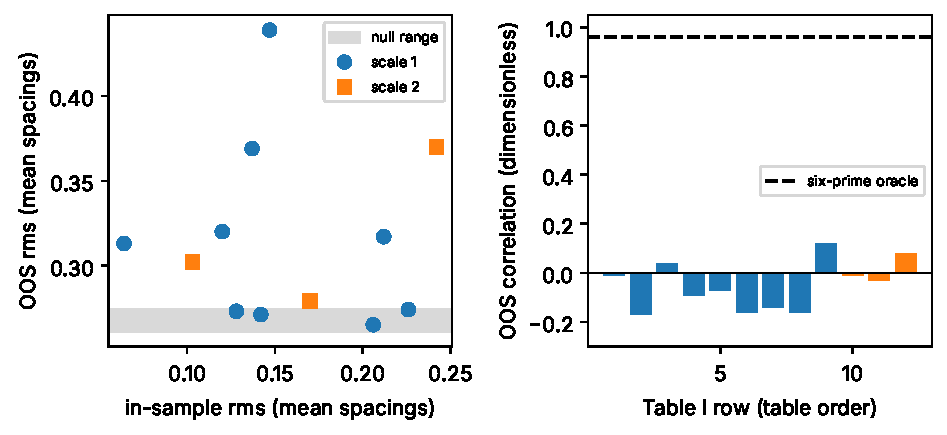
\includegraphics[width=0.85\linewidth]{figs/paper-memorization_tableI.pdf}
\caption{Paper Table~I drawn as a picture. Left: OOS rms against in-sample rms for the twelve configurations (circles: scale 1; squares: scale 2); the shaded band is the range of null references 0.261--0.274 quoted in the table caption. Every point lies in or above the band, wherever it sits horizontally. Right: OOS correlation for each row (in table order); the dashed line is the six-prime explicit-formula oracle's correlation $+0.96$ on zeros 401--500 (paper Table~V).}
\label{fig:paper-memorization-tableI}
\end{figure}

Three features stand out in \cref{fig:paper-memorization-tableI}. First, no point lies below the null band. Second, the horizontal position (in-sample quality) does not predict the vertical one: the best in-sample row (0.064) has OOS 0.313, worse than the null. Third, the correlations scatter around zero, from $-0.17$ to $+0.12$, nowhere near the oracle's $+0.96$.

A compact way to put every row on one scale is a \emph{relative skill}
\begin{equation}
S=1-\frac{\rms_{\rm model}}{\rms_{\rm null}} .
\label{eq:paper-memorization-skill}
\end{equation}
This is our convenience, not a quantity the paper reports. $S>0$ means better than doing nothing, $S=0$ means no better, $S<0$ means harm, and $S=1$ means perfect prediction.

\begin{sample}{Relative skill of the operator rows and the oracle}
Compute $S$ for the four 1--400 rows of Table~I that use $M=400$ or $M=600$ without ridge or with $\mu=0.3$, and for the six-prime and one-prime oracles on the same holdout (paper Table~V: rms 0.074 and 0.198). Use the null 0.263.

\textbf{Step 1:} $M=400$: $S=1-0.369/0.263=1-1.403=-0.403$.

\textbf{Step 2:} $M=400$, $\mu=0.3$: $S=1-0.265/0.263=1-1.0076=-0.0076$.

\textbf{Step 3:} $M=600$: $S=1-0.313/0.263=1-1.190=-0.190$.

\textbf{Step 4:} Six-prime oracle: $S=1-0.074/0.263=1-0.281=+0.719$.

\textbf{Step 5:} One-prime oracle: $S=1-0.198/0.263=1-0.753=+0.247$.

\[
\boxed{S_{M=400}=-0.40,\quad S_{\mu=0.3}=-0.008,\quad S_{M=600}=-0.19,\quad S_{6\,\text{primes}}=+0.72,\quad S_{\{2\}}=+0.25}
\]
The best operator row is essentially at zero skill; the explicit formula with a single prime and no fitted parameters already has positive skill. This is the comparison behind paper Fig.~1 and the statement in Sec.~IV that one prime beats every fitted operator's holdout performance by a factor of at least about 1.3 ($0.265/0.198=1.34$).
\end{sample}

\paragraph{Fluctuations that are there but wrong.} The paper says: ``The fitted models emit fluctuations of $0.16$--$0.62\times$ the true amplitude that are uncorrelated with truth.'' This sentence explains why the OOS rms sits above the null rather than at it. The next sample problem derives the relation.

\begin{sample}{Why an uncorrelated prediction is worse than the null}
Let the held-out truth have values $d_n$ and the prediction have values $p_n$, with means $\bar d$, $\bar p$, standard deviations $\sigma_d$, $\sigma_p$ and correlation $\rho$. (a) Express the mean square error in these quantities. (b) If $\bar p=0$ and $\rho=0$, and the prediction amplitude is $a$ times the null rms, how does the OOS rms compare with the null? Evaluate for $a=0.16$ and $a=0.62$ with null 0.263. (c) What correlation is needed to beat the null when $\bar p=\bar d=0$?

\textbf{Step 1:} Write the error $e_n=p_n-d_n$, and write each variable as mean plus deviation: $p_n=\bar p+p_n'$, $d_n=\bar d+d_n'$, where the deviations average to zero. Denote averages over $\mathcal H$ by $\langle\cdot\rangle$.

\textbf{Step 2:} Expand the square:
\[
\langle e^2\rangle=\langle p^2\rangle-2\langle pd\rangle+\langle d^2\rangle .
\]

\textbf{Step 3:} Each term, using $\langle p'\rangle=\langle d'\rangle=0$:
\[
\langle p^2\rangle=\bar p^2+\sigma_p^2,\qquad
\langle d^2\rangle=\bar d^2+\sigma_d^2,\qquad
\langle pd\rangle=\bar p\bar d+\langle p'd'\rangle=\bar p\bar d+\rho\sigma_p\sigma_d ,
\]
where the last step is the definition of the Pearson correlation, $\rho=\langle p'd'\rangle/(\sigma_p\sigma_d)$ (Chapter~\ref{ch:probability}).

\textbf{Step 4:} Substitute and collect $\bar p^2-2\bar p\bar d+\bar d^2=(\bar p-\bar d)^2$:
\begin{equation}
\langle e^2\rangle=(\bar p-\bar d)^2+\sigma_p^2+\sigma_d^2-2\rho\,\sigma_p\sigma_d .
\label{eq:paper-memorization-decomp}
\end{equation}

\textbf{Step 5:} For (b), set $\bar p=0$ and $\rho=0$: $\langle e^2\rangle=\bar d^2+\sigma_d^2+\sigma_p^2=\rms_{\rm null}^2+\sigma_p^2$, using Eq.~\eqref{eq:paper-memorization-null}. With $\sigma_p=a\,\rms_{\rm null}$,
\[
\rms=\rms_{\rm null}\sqrt{1+a^2}.
\]

\textbf{Step 6:} Numbers: $a=0.16$ gives $0.263\sqrt{1.0256}=0.263\times1.0127=0.2663$; $a=0.62$ gives $0.263\sqrt{1.3844}=0.263\times1.1766=0.3094$.

\textbf{Step 7:} For (c), with zero means, $\langle e^2\rangle<\sigma_d^2$ requires $\sigma_p^2-2\rho\sigma_p\sigma_d<0$, that is (dividing by $\sigma_p\sigma_d>0$) $\rho>\sigma_p/(2\sigma_d)=a/2$.

\[
\boxed{\rms=\rms_{\rm null}\sqrt{1+a^2}:\ 0.266\ (a=0.16)\ \text{to}\ 0.309\ (a=0.62);\qquad \text{beating the null needs}\ \rho>a/2}
\]
\emph{Comment.} The paper's amplitude range accounts for OOS values from 0.266 to 0.309. Some rows of Table~I are higher (0.369, 0.439). By Eq.~\eqref{eq:paper-memorization-decomp}, a larger rms at small $\rho$ needs a larger prediction amplitude in those rows or a mean offset $\bar p-\bar d$. The paper does not report the decomposition row by row, so we cannot say which; Problem~5 explores the arithmetic.
\end{sample}

\paragraph{Regularization: from ``memorize more'' to ``do nothing''.} The paper says regularization ``moves them smoothly from `memorize more' to `do nothing' and never creates skill''. Look at the three 1--400, $M=400$ rows. As the ridge strength goes $\mu=0\to0.03\to0.3$, the in-sample rms rises $0.137\to0.142\to0.206$ and the OOS rms falls $0.369\to0.271\to0.265$, approaching the null 0.263 from above. Recall from Chapter~\ref{ch:least-squares} that the ridge filter shrinks every coefficient toward zero; as $\mu\to\infty$, $c\to0$ and the model \emph{is} the null. Ridge removes the harm done by large uncontrolled coefficients, but it can only interpolate between the unregularized fit and the null; it cannot add information that the parametrization does not carry.

\paragraph{Optimizer variability.} The table caption reports that four random-initialization repeats of the (scale 1, $M=400$, 1--400) row give identical in-sample rms 0.1370 and OOS 0.365--0.379 with correlation $-0.06$ to $-0.08$, and three repeats of the (scale 2, $M=600$) row give OOS 0.279--0.283. The scatter across restarts is small compared with the gap to the oracle. The caption also flags that the scale-2 $M=300$ row needed a relaxed step-acceptance threshold ($1-10^{-5}$ instead of $0.999$, Appendix~A step~6); under the strict rule the optimizer accepts no step and the configuration stays at the null. The paper keeps that row as a sensitivity result, and the conclusion is the same either way.

\paragraph{Uniformity across the holdout.} One might worry that the failure is concentrated at the top of the holdout, where levels approach the edge of the basis coverage or the box. The paper checks: ``Hermitian OOS error is uniform across the holdout (e.g.\ $M=600$, scale 1: rms $0.321/0.304$ on its first/second half), ruling out edge-of-coverage effects.''

\begin{sample}{Do the two halves add up to the table entry?}
The scale-1, $M=600$, fit 1--400 row has OOS rms 0.313 on zeros 401--500. The first half (401--450) has rms 0.321 and the second half (451--500) has 0.304. Check consistency.

\textbf{Step 1:} The mean square over the union of two sets of equal size is the average of the two mean squares, because $\frac{1}{100}\sum_{\rm all}e^2=\frac12\left(\frac{1}{50}\sum_{\rm first}e^2+\frac{1}{50}\sum_{\rm second}e^2\right)$.

\textbf{Step 2:} $0.321^2=0.103041$ and $0.304^2=0.092416$; their average is $0.0977285$.

\textbf{Step 3:} $\sqrt{0.0977285}=0.3126$.

\[
\boxed{\rms_{401\text{--}500}=0.3126\approx0.313}
\]
The halves reproduce the table entry, and neither half is close to the null: the error is spread evenly, not piled up at the far edge.
\end{sample}

\paragraph{Paper Fig.~1.} The paper's first figure shows zeros 370--460 for the scale-1, $M=400$ fit on zeros 1--400. In the training region both the operator and the six-prime formula track the fluctuations; past the boundary the operator's held-out correlation is $-0.07$ (the 1--400, $M=400$ row of Table~I) while the formula's is $+0.96$ (the 401--500 row of Table~V). Neither curve uses any zero past the boundary.

\begin{checkpoint}
In Table~I, the row with the lowest in-sample error (0.064) does not have the lowest OOS error. Which row has the lowest OOS error, and why is that not evidence of skill?
\end{checkpoint}
\checkanswer{The ridge row $\mu=0.3$ (OOS 0.265). It is the row closest to the null model, having been shrunk most toward $c=0$; its OOS rms is still slightly above the null 0.263 and its correlation is $-0.14$. Being near the null is the absence of harm, not the presence of skill.}

\begin{keyideas}
\item In all twelve rows of paper Table~I the OOS rms is at or above the null, and correlations scatter around zero ($-0.17$ to $+0.12$).
\item By Eq.~\eqref{eq:paper-memorization-decomp}, an uncorrelated prediction with nonzero amplitude is always worse than the null; to beat the null a zero-mean prediction needs $\rho>a/2$.
\item Ridge regularization moves the fit toward the null and stops there; restarts change little; errors are uniform across the holdout.
\end{keyideas}

%======================================================================
\section{How sure are we? Bootstrap intervals}\label{sec:paper-memorization-bootstrap}

A table entry computed on 100 held-out zeros is a sample statistic; a different set of 100 zeros would give a somewhat different number. Recall from Chapter~\ref{ch:controls} the \emph{percentile bootstrap}: draw 100 indices from the held-out set with replacement, recompute rms and correlation, repeat many times, and report the 2.5th and 97.5th percentiles of the resampled values as a 95\% interval. The paper uses $2\times10^4$ resamples (Appendix~A step~13).

The paper's statements (Sec.~III, second paragraph):
\begin{itemize}
\item scale 1, $M=400$, random-restart replicate: OOS rms $[0.33,0.43]$, correlation $[-0.21,+0.08]$;
\item scale 2, $M=600$: OOS rms $[0.26,0.30]$, correlation $[-0.18,+0.08]$;
\item six-prime oracle on the same 401--500 holdout: correlation $[+0.95,+0.97]$.
\end{itemize}

\paragraph{How to read them.} For scale 1, the whole rms interval lies above 0.263, so the paper says the fit is ``significantly worse than the null''. For scale 2, the interval $[0.26,0.30]$ contains 0.274: the fit is ``consistent with its null'', meaning indistinguishable from doing nothing. Both correlation intervals contain zero and lie far below the oracle's interval. Nothing in these intervals points toward skill.

\begin{beyond}
The percentile bootstrap gives approximately correct coverage when the resampled units are independent and identically distributed and the sample is not too small; the theory is in Efron and Tibshirani \cite{efron}. We take that result on trust. The fluctuations $d_n$ are \emph{not} independent: consecutive values are correlated (Section~\ref{sec:paper-memorization-within}). The block bootstrap, which resamples runs of consecutive indices, is the standard repair; its theory is also beyond this book.
\end{beyond}

The paper addresses the dependence directly in the ``Other bases'' paragraph: ``The intervals in Table~II resample held-out levels independently although the fluctuations are serially correlated; recomputed with a moving-block bootstrap (block lengths 3 to 20) they widen slightly and no conclusion changes (for the cosine row, at most $[0.30,0.44]$).'' Appendix~A step~22 records a circular block bootstrap with block lengths 3--20 on zeros 401--500. The Discussion repeats the general caveat: ``Bootstrap intervals resample held-out levels independently except where stated.''

\begin{checkpoint}
The block-bootstrap interval for the cosine row is at most $[0.30,0.44]$, wider than the independent interval. Why does serial correlation widen intervals?
\end{checkpoint}
\checkanswer{Correlated neighbors carry partly redundant information, so 100 correlated levels behave like fewer independent ones. Independent resampling ignores this redundancy and underestimates the variability; resampling blocks keeps neighbors together and recovers the larger spread (Chapter~\ref{ch:controls}).}

\begin{keyideas}
\item The principal scale-1 rms interval $[0.33,0.43]$ excludes the null from below: significantly worse than doing nothing. The scale-2 interval contains its null.
\item Correlation intervals of the fits contain zero; the oracle's is $[+0.95,+0.97]$.
\item Block bootstrap (blocks 3--20) widens intervals slightly and changes no conclusion.
\end{keyideas}

%======================================================================
\section{Other bases}\label{sec:paper-memorization-bases}

A natural objection is that cosines are a poor basis: they are global, so a change of one coefficient moves $\delta V$ everywhere. The paper reruns the protocol with two other bases for the even correction (paper Sec.~II~C, ``Other bases''; Appendix~A step~16), defined in Chapter~\ref{ch:fitting}:
\begin{itemize}
\item \textbf{Chebyshev} polynomials $T_k(2|x|/L-1)$, $k=0,\dots,M-1$: global, with resolution concentrated near $x=0$ and $x=L$. (Notation warning: this $T_k$ is a polynomial, unrelated to the training-window length $T$ or the tensors $T^{(n)}$ of Sec.~V.)
\item \textbf{Hat} functions: piecewise-linear tents on $M$ uniform nodes of $|x|/L$, with local support, ``the simplest stand-in for a wavelet-type basis''.
\end{itemize}
Only the basis changes. Paper Table~II gives the results for fit 1--400, holdout 401--500, null 0.263; \cref{fig:paper-memorization-bases} draws its intervals.

\begin{figure}[htbp]\centering
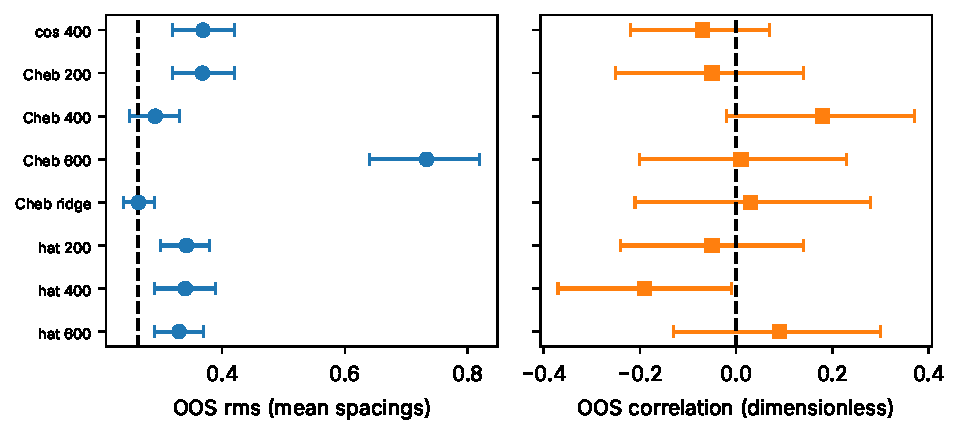
\includegraphics[width=0.85\linewidth]{figs/paper-memorization_bases.pdf}
\caption{Paper Table~II as intervals. Left: OOS rms with bootstrap 95\% intervals for each basis and $M$ (fit 1--400, holdout 401--500); the dashed line is the null 0.263. Right: OOS correlation with its interval; the dashed line is zero. ``Cheb ridge'' is Chebyshev $M=400$ with $\mu=0.3$. All values quoted from the paper.}
\label{fig:paper-memorization-bases}
\end{figure}

\paragraph{What the table shows.} In each basis the in-sample error falls with $M$ (Chebyshev $0.230\to0.162\to0.111$; hat $0.221\to0.145\to0.066$). Every unregularized OOS rms is above 0.263. Ridge with $\mu=0.3$ returns the Chebyshev fit to the null (0.264), as for cosines. The cosine row, 0.369 / $-0.07$, is the Table~I configuration rerun through the alternative-basis code (Appendix~A anchor: 0.1370 / 0.3685 / $-0.0709$), a consistency check between two code paths.

\paragraph{The marginal row.} The paper is careful here, and we should be too. Chebyshev $M=400$ gives OOS rms 0.291 with correlation $+0.18$. The paper says: ``its rms interval contains the null and its correlation interval has its lower end at zero.'' The rms interval is $[0.25,0.33]$ and the correlation interval is $[-0.02,+0.37]$. The paper's verdict has two halves, and both should be kept: ``one such row among eight is not evidence of prediction, but a small positive correlation for this row is not excluded.'' The supporting observation is that the neighbors $M=200$ and $M=600$ show no trend (0.368 and 0.733, correlations $-0.05$ and $+0.01$). If $+0.18$ reflected real structure that Chebyshev polynomials capture, we would expect it not to vanish when the basis is enlarged.

\paragraph{One interval below zero.} The hat $M=400$ row has correlation $-0.19$ with interval $[-0.37,-0.01]$, which excludes zero from below. The paper does not single this row out. Read at face value it indicates anti-skill, a prediction that tends to go the wrong way; Section~\ref{sec:paper-memorization-within} gives a mechanism by which fitted interpolants can be anticorrelated with the truth. Whatever its cause, a negative correlation is not predictive skill.

\begin{checkpoint}
Of the eight rows in Table~II, how many have an OOS rms interval lying entirely above the null 0.263?
\end{checkpoint}
\checkanswer{Six: cosine 400 $[0.32,0.42]$, Chebyshev 200 $[0.32,0.42]$, Chebyshev 600 $[0.64,0.82]$, hat 200 $[0.30,0.38]$, hat 400 $[0.29,0.39]$, hat 600 $[0.29,0.37]$. The other two (Chebyshev 400 $[0.25,0.33]$ and Chebyshev ridge $[0.24,0.29]$) contain the null. None lies below it.}

\begin{keyideas}
\item Chebyshev and hat bases reproduce the cosine pattern: in-sample error falls with $M$, OOS error stays above the null, ridge returns to the null.
\item Chebyshev $M=400$ (0.291, $+0.18$) is marginal: not evidence of prediction, but a small positive correlation is not excluded. Keep both halves of the hedge.
\end{keyideas}

%======================================================================
\section{Within-height splits}\label{sec:paper-memorization-within}

\paragraph{The worry: covariate shift.} Every split in Table~I trains on low zeros and tests on higher ones. Recall from Chapter~\ref{ch:generalization} that when test data come from a different region than training data (covariate shift), failure can reflect the shift rather than a failure to learn. Here the fluctuation amplitude grows slowly with height: the null grows from 0.263 to 0.296 across paper Table~V. To rule this out, the paper also trains and tests \emph{within one height range} (paper Sec.~II~C, ``Within-height splits''; Appendix~A step~17):
\begin{itemize}
\item random 80/20 splits: 20\% of the indices chosen at random are held out (ten seeds at scale 1 inside zeros 1--400; two seeds at scale 2 inside zeros 1--800);
\item odd/even splits: train on odd-indexed zeros and score on even-indexed ones, or the reverse.
\end{itemize}

\paragraph{Results (paper Table~III).} ``The random 80/20 splits are the principal evidence: every held-out error is above the null, by a factor $1.5$--$3.0$ at scale~1 and $1.8$--$1.9$ at scale~2, and no correlation is reliably positive.'' On the same held-out sets the six-prime oracle scores 0.062--0.063 with correlation $+0.97$. The table caption stresses that the seeds reuse the same zeros, so the ranges indicate robustness and are not standard errors.

\paragraph{Saturation.} An odd/even split at scale 1 has 200 training levels. A model with $M\ge200$ coefficients can fit 200 numbers exactly (Chapter~\ref{ch:least-squares}), so those rows are \emph{saturated}: the in-sample rms of the $M=400$ odd and even rows is below $10^{-3}$. The paper calls these rows ``stress tests of memorization''. Saturation is a statement about the count of unknowns, not a guarantee that the optimizer finds an exact fit. The $M=200$ odd and even rows are nominally saturated ($200\ge200$), yet they reach in-sample rms only 0.176 and 0.171: the damped, accept-only-improvements iteration stops well before the residuals vanish, and a linearized problem with exactly as many unknowns as equations can be poorly conditioned. The informative odd/even rows are those with $M=100$, fewer coefficients than levels: held-out errors 0.312 and 0.311 against nulls 0.238 and 0.250, still above the null.

\paragraph{Worse within height.} The paper notes: ``The failure is in fact worse within height than in forward extrapolation.'' Compare the random-split held-out errors at scale 1, $M=400$ (0.50--0.71) with the forward 1--400 row of Table~I (0.369). Section~\ref{sec:paper-memorization-gap} gives the mechanism: the fit does damage in the parts of the potential probed only by the held-out levels.

\paragraph{Why the correlations are negative.} The odd/even rows at $M\le200$ have correlations $-0.26$ to $-0.39$. The paper explains: ``The negative correlations at $M\le200$ are mechanical: the fluctuation sequence has negative autocorrelation at lags 1--3, so any smooth interpolation between neighbouring training levels is anticorrelated with the truth (the mean of the two nearest training fluctuations gives $-0.26$ to $-0.41$).'' The next sample problem makes this mechanism quantitative.

\begin{sample}{Mechanical anticorrelation of neighbor averages}
Treat the fluctuations $d_n$ as a stationary sequence with mean zero, variance $\sigma^2$ and autocorrelations $\rho_1$, $\rho_2$ at lags 1 and 2. (a) Show that the prediction $q_n=\tfrac12(d_{n-1}+d_{n+1})$ has correlation $\rho_1/\sqrt{(1+\rho_2)/2}$ with $d_n$. (b) Estimate $\rho_1$ from the GUE spacing variance and the null $\sigma=0.263$. (c) Evaluate the correlation of (a) for the illustrative values $\rho_1=-0.29$, $\rho_2=-0.10$.

\textbf{Step 1:} Covariance of prediction and truth:
\[
\mathrm{Cov}(q_n,d_n)=\tfrac12\left[\mathrm{Cov}(d_{n-1},d_n)+\mathrm{Cov}(d_{n+1},d_n)\right]=\tfrac12[\rho_1\sigma^2+\rho_1\sigma^2]=\rho_1\sigma^2 .
\]

\textbf{Step 2:} Variance of the prediction:
\[
\mathrm{Var}(q_n)=\tfrac14\left[\mathrm{Var}(d_{n-1})+\mathrm{Var}(d_{n+1})+2\,\mathrm{Cov}(d_{n-1},d_{n+1})\right]=\tfrac14[2\sigma^2+2\rho_2\sigma^2]=\tfrac{1+\rho_2}{2}\sigma^2,
\]
since $d_{n-1}$ and $d_{n+1}$ are two steps apart.

\textbf{Step 3:} Correlation is covariance over the product of standard deviations:
\begin{equation}
\corr(q,d)=\frac{\rho_1\sigma^2}{\sigma\sqrt{(1+\rho_2)/2}\;\sigma}=\frac{\rho_1}{\sqrt{(1+\rho_2)/2}} .
\label{eq:paper-memorization-nbrcorr}
\end{equation}
Its sign is the sign of $\rho_1$: if neighbors are negatively correlated, averaging them predicts the wrong direction.

\textbf{Step 4:} For (b), consider the difference of consecutive fluctuations. Since $s_{n+1}-s_n\approx\gap_n$ and $\gap$ varies slowly,
\[
d_{n+1}-d_n\approx\frac{t_{n+1}-t_n}{\gap_n}-\frac{s_{n+1}-s_n}{\gap_n}\approx u_n-1,
\]
where $u_n$ is the unfolded spacing, of mean 1 (Chapter~\ref{ch:level-statistics}).

\textbf{Step 5:} Take variances. On the left, by stationarity, $\mathrm{Var}(d_{n+1}-d_n)=\sigma^2+\sigma^2-2\rho_1\sigma^2=2\sigma^2(1-\rho_1)$. On the right, $\mathrm{Var}(u_n-1)=\mathrm{Var}(u)$. Solving,
\begin{equation}
\rho_1\approx1-\frac{\mathrm{Var}(u)}{2\sigma^2}.
\label{eq:paper-memorization-rho1}
\end{equation}

\textbf{Step 6:} For the GUE Wigner surmise $p(u)=\frac{32}{\pi^2}u^2e^{-4u^2/\pi}$, the second moment is $\langle u^2\rangle=\frac{32}{\pi^2}\int_0^\infty u^4e^{-4u^2/\pi}\dd u$. With the Gaussian moment $\int_0^\infty u^4e^{-\alpha u^2}\dd u=\frac38\sqrt\pi\,\alpha^{-5/2}$ and $\alpha=4/\pi$, we get $\alpha^{-5/2}=\pi^{5/2}/32$ and
\[
\langle u^2\rangle=\frac{32}{\pi^2}\cdot\frac38\sqrt\pi\cdot\frac{\pi^{5/2}}{32}=\frac{3\pi^3}{8\pi^2}=\frac{3\pi}{8}=1.1781 .
\]
So $\mathrm{Var}(u)=1.1781-1=0.1781$.

\textbf{Step 7:} With $\sigma=0.263$, $2\sigma^2=0.13834$, and Eq.~\eqref{eq:paper-memorization-rho1} gives $\rho_1\approx1-0.1781/0.13834=1-1.287=-0.287$.

\textbf{Step 8:} For (c), $\sqrt{(1-0.10)/2}=\sqrt{0.45}=0.6708$, and $-0.29/0.6708=-0.432$.

\[
\boxed{\corr(q,d)=\frac{\rho_1}{\sqrt{(1+\rho_2)/2}},\qquad \rho_1\approx-0.29,\qquad \corr\approx-0.43\ \text{for}\ \rho_2=-0.10}
\]
\emph{Status.} Step 7 is a heuristic estimate: it uses the Wigner surmise instead of the exact distribution of the zeros, assumes stationarity, and borrows $\sigma$ from the holdout. The value $\rho_2=-0.10$ is illustrative only. The point is the sign: because the spacing variance exceeds $2\sigma^2$, the lag-1 autocorrelation must be negative. Problem~15 asks you to measure the actual autocorrelations; the paper states only that they are negative at lags 1--3. The illustrative $-0.43$ happens to be of the same order as the paper's measured $-0.26$ to $-0.41$, but this is not a test: $\rho_2$ was chosen by hand, and the paper's values are measured on held-out subsets with training neighbors. Step 4 adds two further approximations: $\gap$ is treated as constant between neighbors, and $d_n$ is treated as stationary although its variance grows slowly with $n$. The real autocorrelations are measured in Problem~15.
\end{sample}

\begin{figure}[htbp]\centering
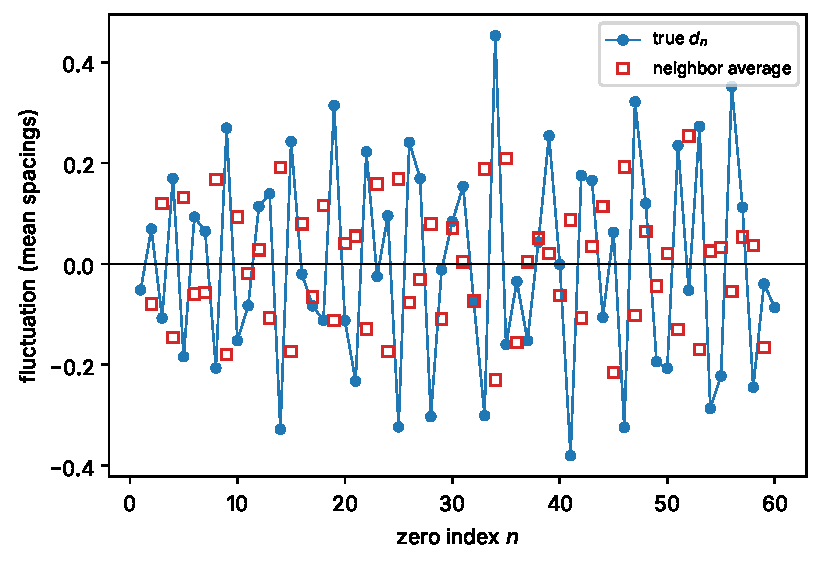
\includegraphics[width=0.85\linewidth]{figs/paper-memorization_neighbors.pdf}
\caption{The first 60 fluctuations $d_n=(t_n-s_n)/\gap_n$ (filled circles, in mean spacings, computed from the true zeros) and the neighbor-average prediction $\tfrac12(d_{n-1}+d_{n+1})$ (open squares). Where a zero sits high, its neighbors tend to sit low, so their average tends to point the wrong way. This is the ``mechanical'' anticorrelation of paper Sec.~III.}
\label{fig:paper-memorization-neighbors}
\end{figure}

\paragraph{The structure is usable, by the right predictor.} A negative $\rho_1$ is information, and a predictor that learns its sign can use it. Recall \emph{simple kriging} from Chapter~\ref{ch:generalization}: the best linear predictor of a held-out value from training values, built from the estimated autocovariance. For two neighbors, the best weight on their average has the sign of $\rho_1$, so kriging turns anticorrelation into positive correlation (Problem~13). The paper reports that within one height range, kriging from the training fluctuations predicts held-out true zeros at 0.117 with correlation $+0.87$ (Sec.~III, surrogate paragraph). Its construction is recorded honestly in Appendix~A step~19: autocovariance to lag 40, a $\cos^2$ taper, a positive-semidefinite projection and a nugget 0.05, with the projection and nugget ``added once, after a first version without them was numerically unstable, and not tuned''. The fitted potential, held out in the same way, does not achieve this.

\begin{checkpoint}
Why are the odd/even rows with $M=400$ at scale 1 not counted as evidence against the operator family, even though their held-out errors (0.351, 0.368) are well above the nulls?
\end{checkpoint}
\checkanswer{With 200 training levels and 400 coefficients the fit is saturated: the system is underdetermined and has infinitely many exact solutions, so the held-out behavior is set by which solution the optimizer happens to pick. Any family would memorize there. The paper uses these rows as stress tests; the evidence comes from the random 80/20 splits and the $M=100$ odd/even rows.}

\begin{keyideas}
\item Within-height random 80/20 splits remove covariate shift; held-out errors remain 1.5--3.0 (scale 1) and 1.8--1.9 (scale 2) times the null, while the oracle scores 0.062--0.063 with correlation $+0.97$.
\item Odd/even rows with $M$ at or above the number of training levels are saturated; the $M=100$ rows still lose to the null.
\item Consecutive fluctuations are negatively correlated, so smooth interpolation is anticorrelated with truth, Eq.~\eqref{eq:paper-memorization-nbrcorr}; kriging, which learns the sign, reaches 0.117 / $+0.87$.
\end{keyideas}

%======================================================================
\section{Permutation and surrogate tests}\label{sec:paper-memorization-surrogates}

If a model's in-sample accuracy reflects the special structure of the zeros, then destroying that structure should make the fit worse. If the accuracy reflects only capacity, the fit should be just as good on any sequence of the same size. Surrogate data turn this idea into a test (Chapter~\ref{ch:controls}).

\paragraph{The three surrogates.} The paper takes the training fluctuations $d_n$ of zeros 1--400 (in mean spacings, Appendix~A step~18) and replaces them by:
\begin{enumerate}
\item a \textbf{random permutation}: the same values in shuffled order. It keeps the marginal distribution (the histogram of values) and destroys all serial structure;
\item a \textbf{phase-randomized surrogate} \cite{theiler}: Fourier transform, replace each phase by a uniform random phase, transform back. It keeps the power spectrum exactly, hence (by the Wiener--Khinchin connection of Chapter~\ref{ch:fourier-transform}) the circular autocorrelation, and has no arithmetic content;
\item an \textbf{amplitude-adjusted (IAAFT) surrogate} \cite{schreiber}: an iteration that keeps the marginal exactly and the spectrum to about 1\%.
\end{enumerate}
New targets are formed as $E_n[\text{smooth}]+d'_n\gap_n$, with $d'_n$ the surrogate, and the scale-1, $M=400$ protocol is refit.

\begin{pycode}
import numpy as np, qmnt
n = np.arange(1, 401)
d = qmnt.fluct(qmnt.zeros(400), n)        # true fluctuations, mean spacings
rng = np.random.default_rng(1)

perm = rng.permutation(d)                 # surrogate 1: same values, shuffled

D = np.fft.rfft(d)                        # surrogate 2: phase randomization
ph = rng.uniform(0, 2*np.pi, len(D))
ph[0] = 0.0; ph[-1] = 0.0                 # keep mean and Nyquist terms as they are
d_phase = np.fft.irfft(D*np.exp(1j*ph), n=len(d))

for name, a in [("true", d), ("perm", perm), ("phase", d_phase)]:
    print(name, qmnt.rms(a))              # all three rms values agree
\end{pycode}

The listing shows the property that makes these surrogates fair: all three sequences have the same rms (the permutation trivially; the phase surrogate by Parseval's theorem of Chapter~\ref{ch:fourier-series}, since the moduli $|D_k|$ are unchanged). The fit faces targets of identical amplitude; only the structure differs.

\paragraph{Results.} ``Over ten draws each, the in-sample rms is $0.134\pm0.010$, $0.141\pm0.006$, and $0.138\pm0.005$, against $0.137$ for the true zeros and $0.244$ for the null.''

\begin{sample}{Is the true-zero fit special?}
Compare the in-sample rms on the true zeros, 0.137, with each surrogate ensemble. Read ``$\pm$'' as the spread over the ten draws (the paper does not say whether it is a standard deviation or a standard error; Problem~23 shows the conclusion does not depend on this). Also compute the fraction of the null removed in-sample for the true zeros and for the permutation.

\textbf{Step 1:} Permutation: $|0.137-0.134|/0.010=0.30$ spreads.

\textbf{Step 2:} Phase-randomized: $|0.137-0.141|/0.006=0.67$ spreads.

\textbf{Step 3:} IAAFT: $|0.137-0.138|/0.005=0.20$ spreads.

\textbf{Step 4:} Fraction of the null removed, true zeros: $(0.244-0.137)/0.244=0.107/0.244=0.439$.

\textbf{Step 5:} Permutation: $(0.244-0.134)/0.244=0.110/0.244=0.451$.

\[
\boxed{\text{true zeros within }0.2\text{--}0.7\text{ spreads of every surrogate;\ fit removes }44\%\text{ (true) vs }45\%\text{ (shuffled)}}
\]
The fit removes as large a fraction of a shuffled sequence as of the real one. Its in-sample accuracy therefore cannot be attributed to the structure of the zeros. In the paper's words: ``in-sample accuracy measures capacity, not captured structure.''
\end{sample}

\paragraph{A revision note on units.} The paper is open about a change: ``The original submission permuted fluctuations in energy units, which also moves amplitude across heights and gave $0.148$, $0.149$; the spacing-unit convention used here is the cleaner control.'' The point is that a fluctuation of one energy unit is a different number of spacings at different heights, because $\gap_n$ shrinks with $n$. Shuffling energy-unit values therefore mixes amplitude between low and high levels. Shuffling spacing-unit values preserves amplitude everywhere. The older values (Appendix~A anchors 0.1483 and 0.1493 for seeds 1 and 2) are only slightly worse than the true-zero fit, so the conclusion survives either convention.

\paragraph{The held-out variant.} The paper adds a held-out version (one split seed, five draws): kriging predicts held-out true zeros at 0.117 / $+0.87$ and permuted targets at the null, as a structure-learning method should, ``whereas the fitted operator, held out in the same way, fails alike on true zeros and on surrogates ($0.57$--$0.70$; one split, illustrative)''. Note the hedge ``one split, illustrative''; this is supporting evidence, not a systematic study.

\begin{checkpoint}
Kriging on permuted targets scores at the null. Why is that the \emph{desired} behavior for a method that learns structure?
\end{checkpoint}
\checkanswer{A permutation destroys serial correlation, so the training values carry no information about a held-out value at a given position. A method that predicts by exploiting serial correlation should find nothing to exploit and fall back to the null. Failing on permuted data while succeeding on true data is the signature of learning real structure.}

\begin{keyideas}
\item The fit reaches the same in-sample rms on shuffled, phase-randomized and IAAFT surrogates (0.134, 0.141, 0.138) as on the true zeros (0.137).
\item Surrogates are amplitude-matched, so the comparison isolates structure from capacity.
\item Kriging distinguishes true from permuted targets; the operator does not.
\end{keyideas}

%======================================================================
\section{The interpolation split: damage at the turning points}\label{sec:paper-memorization-gap}

\paragraph{The experiment.} Train on zeros 1--200 together with 301--500, and predict the interior gap 201--300 (Appendix~A step~14). The held-out levels are surrounded by training levels on both sides, the most favorable setting for any model that has captured smooth structure.

\paragraph{Results.} In-sample rms 0.136, but a gap error of 2.64 spacings, ``ten times the null $0.255$'', with correlation $-0.02$. Two fits from random starts give gap errors 2.78 and 2.43 with the largest correction at the same position. Ridge refits bring the gap error back to the null: 0.262 at $\mu=0.03$ and 0.257 at $\mu=0.3$, with correlations $-0.02$ and $-0.06$ (Appendix~A step~21).

The ratio is $2.64/0.255=10.4$: the unregularized fit does not merely fail to help; it actively harms the held-out levels.

\paragraph{The mechanism: position maps to level index.} Recall from Chapter~\ref{ch:wkb} that a semiclassical level of energy $E$ is confined between turning points $\pm x_E$ where $V(x_E)=E$, and that it is most sensitive to the potential near those turning points (where the particle moves slowest and $|\psi|^2$ is largest). For the Wu--Sprung potential the turning point of level $n$ is $x(t_n)$, with $x(V)$ from paper Eq.~(2):
\begin{equation}
x(V)=\frac1\pi\left[\sqrt{V-V_0}\,\log\frac{V_0}{2\pi e^2}+\sqrt V\,\log\frac{\sqrt V+\sqrt{V-V_0}}{\sqrt V-\sqrt{V-V_0}}\right],\qquad V_0=3.10073\pi .
\label{eq:paper-memorization-ws}
\end{equation}

\begin{sample}{Turning points on the Wu--Sprung potential}
(a) Evaluate Eq.~\eqref{eq:paper-memorization-ws} at $V=1000$ and confirm the scale-1 half-width $L=44.883$. (b) Evaluate it at $V=500$, the height of the smooth potential where the paper's largest $|\delta V|$ occurs. (c) Compare with the turning band 22.5--28.5 the paper gives for levels 201--300.

\textbf{Step 1:} Constants: $V_0=3.10073\times3.14159=9.74123$. Also $2\pi e^2=6.28319\times7.38906=46.4268$, so $V_0/(2\pi e^2)=0.209819$ and $\log0.209819=-1.56151$.

\textbf{Step 2:} A useful identity for the second logarithm: multiply numerator and denominator by $\sqrt V+\sqrt{V-V_0}$ and use $(\sqrt V)^2-(\sqrt{V-V_0})^2=V_0$:
\[
\frac{\sqrt V+\sqrt{V-V_0}}{\sqrt V-\sqrt{V-V_0}}=\frac{\left(\sqrt V+\sqrt{V-V_0}\right)^2}{V_0}.
\]
This avoids subtracting two nearly equal square roots.

\textbf{Step 3:} $V=1000$: $\sqrt{990.259}=31.4684$, $\sqrt{1000}=31.6228$, sum $63.0912$, squared $3980.50$, divided by $V_0$: $408.62$, logarithm $6.01278$.

\textbf{Step 4:} Bracket: $31.4684\times(-1.56151)+31.6228\times6.01278=-49.138+190.141=141.003$. Divide by $\pi$: $x(1000)=44.883$, the paper's $L$.

\textbf{Step 5:} $V=500$: $\sqrt{490.259}=22.1418$, $\sqrt{500}=22.3607$, sum $44.5025$, squared $1980.47$, divided by $V_0$: $203.31$, logarithm $5.31473$.

\textbf{Step 6:} Bracket: $22.1418\times(-1.56151)+22.3607\times5.31473=-34.575+118.841=84.266$. Divide by $\pi$: $x(500)=26.82$.

\[
\boxed{x(1000)=44.883,\qquad x(500)=26.82\in[22.5,\,28.5]}
\]
The position of the largest fitted correction, where $V\approx500$, lies inside the band of turning points of the held-out levels 201--300. (Problem~11 repeats this for $t_{100}$, and the CHECKS script confirms that $x(t_{201})\approx22.5$ and $x(t_{300})\approx28.5$ from the actual zeros.)
\end{sample}

\begin{figure}[htbp]\centering
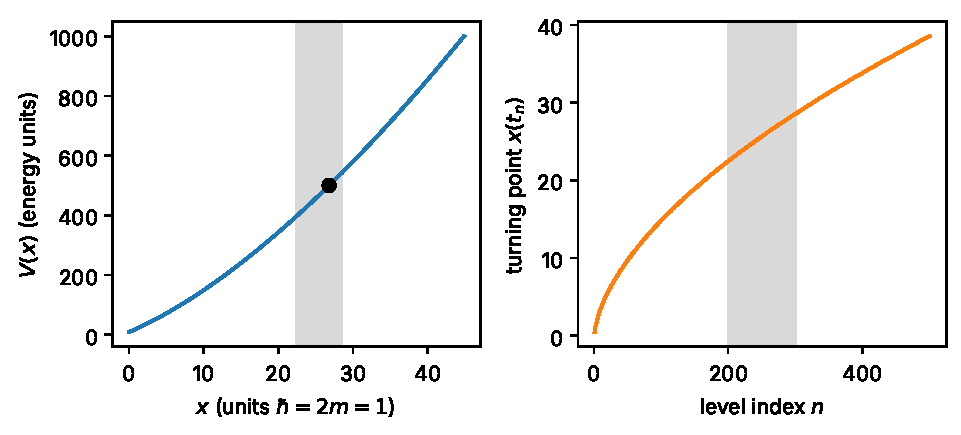
\includegraphics[width=0.85\linewidth]{figs/paper-memorization_turning.pdf}
\caption{Left: the Wu--Sprung potential $V(x)$ for $0\le x\le L=44.883$ (units $\hbar=2m=1$); the shaded band $22.5\le x\le28.5$ contains the turning points of levels 201--300, the held-out gap of the interpolation split; the dot marks $V=500$ at $x=26.82$. Right: turning point $x(t_n)$ against level index $n$ for the first 500 zeros, with the held-out gap shaded. Each level ``owns'' a position on the potential.}
\label{fig:paper-memorization-turning}
\end{figure}

\paragraph{What the fit did.} Paper Fig.~4 shows the single deterministic fit from $c=0$: (a) fitted and smooth potentials, (b) the correction $\delta V$, (c) true and predicted fluctuations. The paper's wording is: ``rms $\delta V = 40$ in that band against $15$ inside it and $13$ outside it, with a maximum $|\delta V| = 199$ where the smooth potential is about $500$''; the predicted gap levels are displaced by $-6$ to $+2$ spacings. The phrase ``inside it'' is ambiguous as written, since the band itself is where the rms is 40. The most natural reading, which we adopt only tentatively, is that 15 refers to the region on the inner side of the band ($x<22.5$) and 13 to the region outside it ($x>28.5$); the paper does not define the regions further. On any reading, the correction in the band is about $40/15=2.7$ and $40/13=3.1$ times its rms in the two comparison regions, and its peak is about $199/500=40\%$ of the local potential.

\paragraph{Why it costs nothing in-sample.} The paper states the conclusion but not a detailed mechanism. What follows in this paragraph, up to the quotation, is our own heuristic reading, not the paper's, and we have not tested it. Training levels with turning points below 22.5 are confined inside the band's inner edge and feel the band only through the exponentially small tails of their wavefunctions in the forbidden region. Training levels 301--500 turn beyond 28.5, so the band lies inside their classically allowed region, where $|\psi|^2$ oscillates rapidly. Their shifts $\int|\psi_n|^2\delta V\,\dd x$ still feel a correction there; it would leave them unchanged only if its contributions largely averaged out against the oscillating densities, or were offset by structure elsewhere that the optimizer adjusts at the same time. Whether the fitted $\delta V$ is of that kind is not reported in the paper (its Fig.~4 shows only the shape), so this part of the argument is speculation. The optimizer, which sees only in-sample residuals, has no reason to keep $\delta V$ small there. In the paper's words: ``The optimizer places large structure in the part of the potential that only the held-out levels probe strongly, because doing so costs nothing in-sample.'' This explanation is heuristic, as is the paper's.

\paragraph{The paper's hedge.} The paragraph ends: ``The unregularized fit is harmful between its training blocks and the regularized fits tried are uninformative there; this does not show that the family could not interpolate under another fitting procedure.'' Keep it. The experiment tests the family \emph{together with} its optimizer.

\paragraph{The forward split, viewed the same way.} The same geometry applies to the forward splits of Table~I, as our own reading (the paper states the mechanism for the interpolation split only). Using Eq.~\eqref{eq:paper-memorization-ws}, $x(680)=33.82$ and $x(811.18)=38.53$: the training levels 1--400 turn inside $|x|\lesssim33.8$, while the held-out levels 401--500 turn in $33.8\lesssim|x|\lesssim38.5$, a region the training levels reach only through forbidden-region tails. The fit's behavior there is again unconstrained by the data.

\begin{checkpoint}
Ridge regularization brings the gap error from 2.64 back to about 0.26. Does the ridge-regularized fit therefore predict the gap?
\end{checkpoint}
\checkanswer{No. 0.262 and 0.257 are at the null 0.255 (slightly above it), and the correlations are $-0.02$ and $-0.06$. Ridge removed the damage by suppressing the large correction, leaving nearly the unperturbed potential there, which is the null. ``Removes the damage and nothing else,'' as the paper says.}

\begin{keyideas}
\item The interpolation split (train 1--200 and 301--500, predict 201--300) gives gap error 2.64, ten times the null 0.255: the fit does harm.
\item Level $n$ probes the potential most strongly near its turning point $x(t_n)$; levels 201--300 turn at $x=22.5$--$28.5$, where the fitted $\delta V$ is largest.
\item Ridge returns the gap to the null; the paper does not claim that no other procedure could interpolate.
\end{keyideas}

%======================================================================
\section{The arithmetic-continuation probe}\label{sec:paper-memorization-probe}

Every experiment so far uses the real zeros, whose fluctuation is a complicated superposition of many prime frequencies plus whatever the truncation misses. A skeptic could say: perhaps the true fluctuation is simply too complicated for a few hundred coefficients to extrapolate. The continuation probe removes that objection. It is the cleanest single experiment in the paper.

\paragraph{The target.} Replace the true targets by a synthetic fluctuation made solely of the $p=2$ term of paper Eq.~(4), our running example RE2:
\begin{equation}
N^{p=2}_{\rm fl}(t)=-\frac1\pi\sum_{m=1}^{3}\frac{\sin(mt\log2)}{m\,2^{m/2}} .
\label{eq:paper-memorization-re2}
\end{equation}
Appendix~A step~15 defines the synthetic targets $T_n=E_n[\text{smooth}]-N^{p=2}_{\rm fl}(s_n)\,\gap_n$. (The letter $T_n$ is a target here, not a Chebyshev polynomial or a tensor.) The minus sign makes the target fluctuation equal $-N^{p=2}_{\rm fl}(s_n)$ spacings, the same sign convention as real zeros: solving $\Nsm(t)+N_{\rm fl}(t)=n-\tfrac12$ moves the root by $-N_{\rm fl}$ divided by the slope $\Nsm'=1/\gap$. Fit the same family on levels 1--400 and ask whether the fitted operator \emph{continues} the oscillation on levels 401--500.

Why is this a fair test? Because the right answer is known exactly: the oscillation does not stop at level 400, and a function with three known frequencies $\log2$, $2\log2$, $3\log2$ is as simple a target as arithmetic offers.

\begin{sample}{How big is the prime-2 wave?}
Find the long-run rms of RE2, and compare with the probe-null 0.1708 of Appendix~A (the rms of predicting zero fluctuation on levels 401--500 for the synthetic target).

\textbf{Step 1:} The amplitudes are $a_m=1/(m\,2^{m/2})$: $a_1=1/\sqrt2=0.707107$, $a_2=1/4=0.25$, $a_3=1/(3\times2\sqrt2)=0.117851$.

\textbf{Step 2:} The mean square over a window of length $T_w$ in $t$ involves averages of $\sin^2(\omega t)$ and of cross products $\sin(\omega t)\sin(\omega' t)$ with $\omega\neq\omega'$. Using $\sin A\sin B=\tfrac12[\cos(A-B)-\cos(A+B)]$ we write
\[
\sin(\omega t)\sin(\omega' t)=\tfrac12\left[\cos((\omega-\omega')t)-\cos((\omega+\omega')t)\right].
\]
For any $\kappa\neq0$, an antiderivative of $\cos(\kappa t)$ is $\sin(\kappa t)/\kappa$, which vanishes at $t=0$, so $\int_0^{T_w}\cos(\kappa t)\,\dd t=\sin(\kappa T_w)/\kappa$. Applying this with $\kappa=\omega-\omega'$ and with $\kappa=\omega+\omega'$, and dividing by $T_w$,
\[
\frac1{T_w}\int_0^{T_w}\sin(\omega t)\sin(\omega' t)\,\dd t=\frac1{2T_w}\left[\frac{\sin((\omega-\omega')T_w)}{\omega-\omega'}-\frac{\sin((\omega+\omega')T_w)}{\omega+\omega'}\right],
\]
which, because $|\sin|\le1$, is at most $\frac1{2T_w}\left(\frac1{|\omega-\omega'|}+\frac1{\omega+\omega'}\right)$ in magnitude and tends to 0 as $T_w\to\infty$. With $\omega'=\omega$ the identity reads $\sin^2(\omega t)=\tfrac12[1-\cos(2\omega t)]$; using the cosine integral with $\kappa=2\omega$, its average over the window is $\frac12-\frac{\sin(2\omega T_w)}{4\omega T_w}\to\frac12$.

\textbf{Step 3:} So in the long run each term contributes $a_m^2/2$ and the cross terms vanish:
\begin{equation}
\rms\left(N^{p=2}_{\rm fl}\right)\to\frac1\pi\sqrt{\frac12\sum_{m=1}^3a_m^2}.
\label{eq:paper-memorization-re2rms}
\end{equation}

\textbf{Step 4:} $\sum a_m^2=0.5+0.0625+0.0138889=0.5763889$; half is $0.2881944$; square root $0.5368374$; divide by $\pi$: $0.17088$.

\[
\boxed{\rms(\text{RE2})\approx0.1709\quad\text{vs. probe-null }0.1708}
\]
\emph{Status.} Eq.~\eqref{eq:paper-memorization-re2rms} is the long-window limit for continuous $t$. The probe samples RE2 at the 100 irregular points $s_{401},\dots,s_{500}$, which span about 14.5 periods (next sample problem), so it is an approximation; the agreement to $10^{-4}$ shows it is a good one here.
\end{sample}

\begin{sample}{How many levels per period?}
(a) Show that the number of consecutive levels per period of $\sin(t\log2)$ is $\log(t/2\pi)/\log2$. Evaluate at $t=680$ (near zero 400) and $t=811.18$ (zero 500). (b) Estimate how many periods lie in the training window 1--400 and in the holdout 401--500, using $t_1=14.13$, $t_{400}\approx680$ and $t_{500}=811.18$.

\textbf{Step 1:} The period in $t$ is $2\pi/\log2=6.28319/0.693147=9.0647$.

\textbf{Step 2:} The spacing at height $t$ is $\gap=2\pi/\log(t/2\pi)$, Eq.~\eqref{eq:paper-memorization-gap}. Levels per period:
\[
\frac{2\pi/\log2}{2\pi/\log(t/2\pi)}=\frac{\log(t/2\pi)}{\log2}=\log_2\frac{t}{2\pi}.
\]

\textbf{Step 3:} At $t=680$: $\log(680/6.28319)=\log108.225=4.68421$; divided by $0.693147$: $6.758$.

\textbf{Step 4:} At $t=811.18$: $\log129.104=4.86062$; divided by $0.693147$: $7.012$.

\textbf{Step 5:} Periods in training: $(680-14.13)/9.0647=665.87/9.0647=73.5$. In the holdout: $(811.18-680)/9.0647=131.2/9.0647=14.5$.

\[
\boxed{\text{about }6.8\text{--}7.0\ \text{levels per period;\ about 73.5 periods in training, 14.5 in the holdout}}
\]
The training window contains more than seventy full periods of the oscillation. Lack of examples is not the problem.
\end{sample}

\begin{figure}[htbp]\centering
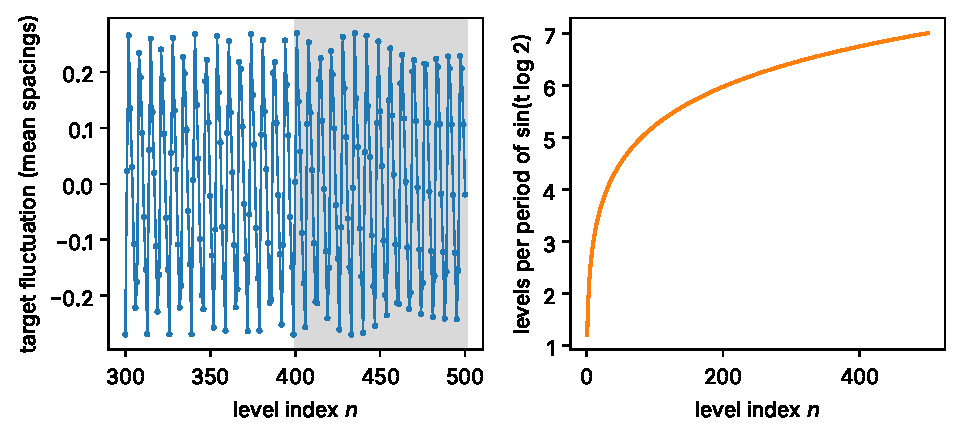
\includegraphics[width=0.85\linewidth]{figs/paper-memorization_probe.pdf}
\caption{The continuation-probe target. Left: the synthetic fluctuation $-N^{p=2}_{\rm fl}(s_n)$ of Eq.~\eqref{eq:paper-memorization-re2} in mean spacings, levels 300--500; the shaded region 401--500 is held out. The correct continuation is the same oscillation. Right: levels per period of $\sin(t\log2)$, $\log_2(t/2\pi)$ evaluated at $t=s_n$, for levels 1--500.}
\label{fig:paper-memorization-probe}
\end{figure}

\paragraph{Results.} ``It represents it almost perfectly in-sample (rms $0.056$, correlation $+0.95$) and continues it not at all (held-out correlation $+0.07$, rms worse than predicting zero fluctuation).'' Appendix~A gives the anchors: in-sample 0.0555, correlation $+0.95$; OOS 0.1958, correlation $+0.07$; probe-null 0.1708. The in-sample rms is about a third of the wave's own rms ($0.0555/0.1709=0.32$), while the OOS rms exceeds the probe-null by $0.1958/0.1708=1.146$, about 15\%.

\paragraph{The contrast: a model that knows the frequency.} Consider instead the six-function model
\[
F(t)=\sum_{m=1}^{3}\left[\beta_m\sin(mt\log2)+\gamma_m\cos(mt\log2)\right],
\]
fitted by least squares to the same 400 target values (Chapter~\ref{ch:sparse-frequency}, control~B). Collect the six functions evaluated at the 400 sample points into the columns of a $400\times6$ matrix $\mathsf F$, and write the target vector as $\mathbf g$. The target is \emph{exactly} in the span: $\mathbf g=\mathsf F\bm\beta_{\rm true}$ with $\beta_m=-1/(\pi m2^{m/2})$ and $\gamma_m=0$. If the six columns are linearly independent (which holds for distinct frequencies sampled at many points), $\mathsf F^\top\mathsf F$ is invertible, and the least-squares solution (Chapter~\ref{ch:least-squares}) is
\[
\hat{\bm\beta}=(\mathsf F^\top\mathsf F)^{-1}\mathsf F^\top\mathbf g=(\mathsf F^\top\mathsf F)^{-1}(\mathsf F^\top\mathsf F)\bm\beta_{\rm true}=\bm\beta_{\rm true}.
\]
The model recovers the exact coefficients, and its prediction at \emph{any} height, in or out of the training window, is the exact wave. Six parameters with the right functional form continue perfectly; a few hundred parameters in a potential do not continue at all.

\paragraph{The paper's interpretation, and its hedges.} Section~III puts it strongly: ``The family can paint one window of $\sin(t\log 2)$ onto its levels but cannot express `continue oscillating': the arithmetic frequency is not in its vocabulary. This is the memorization mechanism exhibited in isolation, on a target where the right continuation is known exactly.'' And: ``the failure on the real zeros is not explained by the complicated mixture of primes in the true fluctuation: a single known arithmetic frequency, learned from a finite window, already defeats the family's extrapolation.''

The Discussion (Sec.~VI) states the scope more carefully: ``Under the fitting protocol used, the parametrizations tested did not recover the long-range continuation of a frequency such as $\log 2$, as the continuation probe shows on a target where the answer is known. This is evidence about the tested parametrizations and optimizer together, not a statement about what a potential can represent.'' A careful reader keeps the second version as the claim. ``Not in its vocabulary'' is an interpretation of an experiment with one background, one basis family at a time and one optimizer; it is not a theorem about potentials. The Discussion also says plainly that ``Whether the memorization result can be derived rather than measured is an open problem.''

Why might a potential not ``speak'' in sinusoids of $t$? Heuristically (the paper's own word): a potential addresses levels through their turning points, locally in energy (Section~\ref{sec:paper-memorization-gap}), whereas the target is an almost-periodic function of $t$, sparse in frequency (Chapter~\ref{ch:fourier-series}). The correction a fit places at the turning points of levels 1--400 says nothing, by itself, about the region $33.8\lesssim x\lesssim38.5$ where levels 401--500 turn.

\paragraph{A small-scale rerun: one linearized step.} The full fit takes minutes per configuration (\texttt{qmnt.fit\_potential}). You can see the shape of the phenomenon in seconds with a linear toy: compute the eigenvectors $\psi_n$ of the Wu--Sprung Hamiltonian once, form $A_{nk}=\int|\psi_n|^2\cos(k\pi x/L)\dd x$ for $n\le500$ and $k<400$, and take a single SVD-damped least-squares step from $c=0$ toward the probe target on levels 1--400. This is the first Gauss--Newton iteration of the paper's fit (Chapter~\ref{ch:fitting}) and nothing more: no iteration, no bias correction, a coarse grid. \Cref{fig:paper-memorization-toy} shows the result; Problem~18 asks you to quantify it and compare with the paper's held-out correlation $+0.07$. Here is the complete toy; the script for \cref{fig:paper-memorization-toy} is the same code plus plotting.

\begin{pycode}
import numpy as np, qmnt
L, N, M = 44.883, 4000, 400
x = qmnt.grid(L, N); h = 2*L/(N+1)
V = np.array([qmnt.wu_sprung_V(abs(xi)) for xi in x])
E, psi = qmnt.fd_levels(V, L, k=500, return_vectors=True)
if psi.shape[0] != N: psi = psi.T            # columns = eigenvectors
dens = psi**2/(np.sum(psi**2, axis=0)*h)     # sum psi^2 h = 1
phi = np.cos(np.outer(x, np.arange(M))*np.pi/L)
A = h*dens.T @ phi                           # A[n,k] = int |psi_n|^2 phi_k dx
n = np.arange(1, 501)
s = qmnt.smooth_zeros(n); g = qmnt.mean_gap(n)
f = -qmnt.Nfl(s, [2])                        # target fluctuation, spacings
U, sig, Wt = np.linalg.svd(A[:400], full_matrices=False)
filt = sig/(sig**2 + 1e-6*sig[0]**2)         # SVD-damped filter
c = Wt.T @ (filt*(U.T @ (f[:400]*g[:400])))  # one step from c = 0
p = (A @ c)/g                                # predicted fluctuation
print('in  ', qmnt.rms(p[:400]-f[:400]), qmnt.corr(p[:400], f[:400]))
print('out ', qmnt.rms(p[400:]-f[400:]), qmnt.corr(p[400:], f[400:]))
print('null', qmnt.rms(f[400:]))
\end{pycode}

\begin{figure}[htbp]\centering
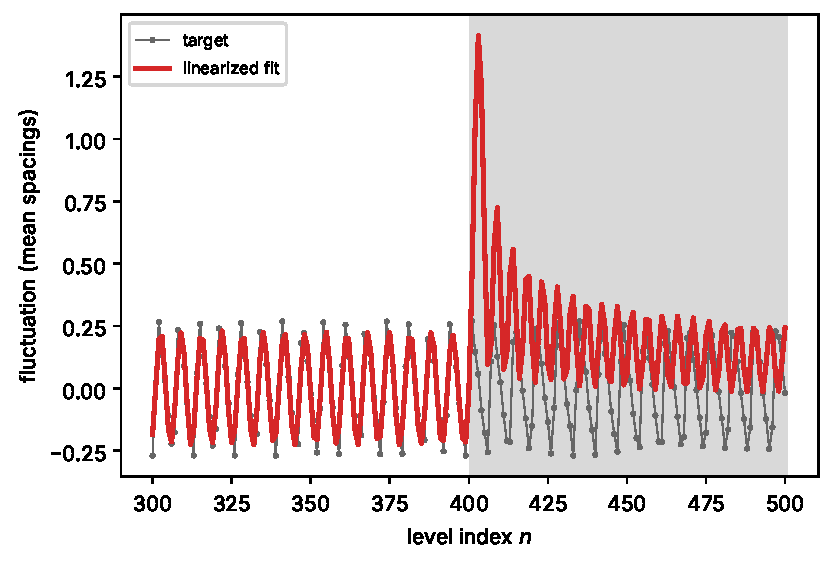
\includegraphics[width=0.85\linewidth]{figs/paper-memorization_toy.pdf}
\caption{A linearized toy of the continuation probe (not the paper's computation). Thin line with dots: the target fluctuation $-N^{p=2}_{\rm fl}(s_n)$ in mean spacings. Thick line: the first-order prediction $\sum_kA_{nk}c_k/\gap_n$ after one SVD-damped least-squares step ($M=400$ cosines, damping $10^{-6}\sigma_1^2$) fitted on levels 1--400 only, using eigenvectors of the Wu--Sprung Hamiltonian on 4000 grid points with $L=44.883$. The shaded region 401--500 was not used. Compare how the prediction behaves on the two sides of the boundary; the paper's full nonlinear fit gives held-out correlation $+0.07$ (Sec.~III).}
\label{fig:paper-memorization-toy}
\end{figure}

\begin{checkpoint}
The probe's in-sample correlation is $+0.95$ and its OOS rms is 0.1958. Why is ``rms worse than predicting zero fluctuation'' a stronger statement than ``correlation $+0.07$''?
\end{checkpoint}
\checkanswer{A correlation near zero says the predicted held-out fluctuation has no linear relation to the truth. The rms comparison adds that the prediction has nonzero amplitude, so by Eq.~\eqref{eq:paper-memorization-decomp} it adds error: the fitted operator does worse than the trivial model that predicts nothing.}

\begin{keyideas}
\item The probe target is RE2 alone, with long-run rms $0.1709$, matching the probe-null 0.1708; the training window holds about 73 of its periods.
\item The fitted family reproduces it in-sample (0.0555, $+0.95$) and does not continue it (0.1958 vs.\ null 0.1708, correlation $+0.07$).
\item A six-function model with the right frequencies recovers the wave exactly from the same data; the obstacle is the form of the model, not the amount of data.
\item The careful statement (paper Sec.~VI) is about the tested parametrizations and optimizer together; deriving the result is open.
\end{keyideas}

%======================================================================
\section{What Section III establishes, and what it does not}\label{sec:paper-memorization-limits}

We now collect the strengths and limits of the section, claim by claim. Chapter~\ref{ch:paper-critique} returns to these from a referee's point of view.

\paragraph{Established within the tested scope.}
\begin{itemize}
\item In-sample agreement with the zeros is achievable at essentially any accuracy by the tested families, and is achieved equally on surrogate targets. In-sample agreement alone is therefore not evidence of captured structure. This is the methodological core, and it is robust: it rests on direct refits, ten draws per surrogate type, and agreement across three surrogate constructions.
\item Across the twelve configurations of Table~I, the eight rows of Table~II, and the within-height splits of Table~III, no row shows reproducible held-out skill relative to the null, while a zero-parameter arithmetic formula shows strong skill on the same holdouts.
\item On a target whose continuation is known exactly (RE2), the tested family under the tested protocol does not continue it.
\end{itemize}

\paragraph{Limits stated by the paper.}
\begin{itemize}
\item One background potential (Wu--Sprung); three bases; Hermite, wavelet and neural-network parametrizations not tested (Secs.~I and VI).
\item Operator fits use at most the first 1000 zeros (Sec.~VI).
\item One Chebyshev row is marginal (Table~II); a small positive correlation for it is not excluded.
\item Bootstrap intervals resample independently except where stated; the block bootstrap was run for Table~II.
\item The interpolation result does not show that the family could not interpolate under another fitting procedure.
\item The explanation of the failure is heuristic; whether it can be derived is open.
\end{itemize}

\paragraph{Things to watch as a reader.}
\begin{itemize}
\item Several results are single-split or few-seed (the surrogate held-out variant: ``one split, illustrative''; scale-2 random splits: two seeds). Ranges over seeds that reuse the same zeros are robustness indications, not standard errors (Table~III caption).
\item The optimizer and the family are tested together. Different stopping rules, priors or regularizers define different procedures, and the paper's conclusions are about the ones it ran.
\end{itemize}

\begin{keyideas}
\item The robust lesson of Section~III is methodological: in-sample spectral agreement demonstrates capacity; held-out tests and surrogate refits are ways to show more, and they are the ones the paper uses.
\item Every specific negative result is scoped to the background, bases and optimizer tested.
\end{keyideas}

%======================================================================
\section{Paper connection}\label{sec:paper-memorization-paper}

\Cref{tab:paper-memorization-map} maps each part of this chapter to the paper (R1 numbering) and to the chapters that supply the tools.

\begin{table}[htbp]\centering
\caption{Where each piece of paper Sec.~III lives, and which chapters explain it.}
\label{tab:paper-memorization-map}
\small
\begin{tabular}{p{3.6cm}p{5.2cm}p{4.2cm}}
\toprule
This chapter & Paper location & Tools \\
\midrule
Protocol recap & Sec.~II A--C; Eqs.~(1), (3); App.~A steps 1--7 & Chs.~\ref{ch:counting-zeros}, \ref{ch:finite-differences}, \ref{ch:fitting} \\
Capacity, coverage law & Sec.~III para.~1; Fig.~3; App.~A anchors $(300,0.186)$, $(900,<10^{-4})$ & Ch.~\ref{ch:fitting} \\
Twelve configurations & Sec.~III para.~2; Table~I; Fig.~1; Fig.~3 & Chs.~\ref{ch:generalization}, \ref{ch:probability} \\
Bootstrap intervals & Sec.~III para.~2 and ``Other bases''; App.~A steps 13, 22 & Ch.~\ref{ch:controls} \\
Other bases & Sec.~II C ``Other bases''; Sec.~III ``Other bases''; Table~II; App.~A step 16 & Chs.~\ref{ch:fitting}, \ref{ch:controls} \\
Within-height splits & Sec.~II C ``Within-height splits''; Sec.~III; Table~III; App.~A steps 17, 19 & Chs.~\ref{ch:generalization}, \ref{ch:level-statistics} \\
Surrogates & Sec.~III ``Permutation and surrogate tests''; App.~A steps 12, 18 & Chs.~\ref{ch:controls}, \ref{ch:fourier-transform} \\
Interpolation split & Sec.~III ``Interpolation split''; Fig.~4; Eq.~(2); App.~A steps 14, 21 & Chs.~\ref{ch:wkb}, \ref{ch:wu-sprung} \\
Continuation probe & Sec.~III ``Arithmetic-continuation probe''; Eq.~(4); App.~A step 15; Sec.~VI & Chs.~\ref{ch:explicit-formula}, \ref{ch:sparse-frequency} \\
\bottomrule
\end{tabular}
\end{table}

\paragraph{Numbers you can reproduce cheaply.} With \texttt{qmnt} (Appendix~A of this book teaches the Python) you can reproduce, in seconds, the null rms 0.263 on zeros 401--500 (paper Sec.~II~C), the six-prime oracle score 0.074 / $+0.96$ (paper Table~V, used in Fig.~1 and throughout Sec.~III), the probe-null 0.1708 (paper App.~A), the turning band 22.5--28.5 (paper Sec.~III), the half-widths $L=44.883$ and $59.957$ (paper Sec.~II~B), and the sign of the fluctuation autocorrelations (paper Sec.~III). The full fits behind Tables~I--III require \texttt{qmnt.fit\_potential} or the Zenodo pipeline \cite{zenodo}.

\begin{pycode}
import numpy as np, qmnt
n = np.arange(401, 501)                       # RE5: the principal holdout
s = qmnt.smooth_zeros(n)
d = qmnt.fluct(qmnt.zeros(500)[n-1], n)
print("null rms", qmnt.rms(d))                # paper: 0.2631

P6 = qmnt.first_primes(6)                     # 2, 3, 5, 7, 11, 13
print("oracle", qmnt.score(qmnt.oracle_zeros(n, P6), n))   # Table V: 0.074 / +0.96

print("probe-null", qmnt.rms(qmnt.Nfl(s, [2])))            # App. A: 0.1708
print("turning band", qmnt.wu_sprung_x(qmnt.zeros(300)[[200, 299]]))  # ~22.5, 28.5
\end{pycode}

\paragraph{Reproducibility record.} Every number in Section~III is regenerated by the scripted pipeline archived on Zenodo \cite{zenodo}, which the author reports rerunning end to end (Appendix~A). The revision computations (steps 16--23) are included in the updated record, and Appendix~A notes that overwriting held-out data with noise before fitting leaves all fitted coefficients bit-identical, a direct check that no held-out zero entered the fit.

%======================================================================
\section{Summary}\label{sec:paper-memorization-summary}

\begin{itemize}
\item Fluctuations are measured as $d_n=(t_n-s_n)/\gap_n$, Eq.~\eqref{eq:paper-memorization-fluct}; scores are the held-out rms and correlation of Eq.~\eqref{eq:paper-memorization-score}; the null predicts $p_n=0$, Eq.~\eqref{eq:paper-memorization-null}, with rms 0.263 on zeros 401--500.
\item Capacity: the cosine family reaches in-sample rms 0.186 at $M=300$ and below $10^{-4}$ at $M=900$ on 500 levels; the heuristic coverage law Eq.~\eqref{eq:paper-memorization-coverage} predicts completeness at $M\gtrsim814$.
\item Transfer: in all twelve configurations of paper Table~I, OOS rms is at or above the null and correlations scatter around zero; relative skill Eq.~\eqref{eq:paper-memorization-skill} is at most about zero, against $+0.72$ for the six-prime oracle.
\item An uncorrelated prediction of relative amplitude $a$ has rms $\rms_{\rm null}\sqrt{1+a^2}$; beating the null needs $\rho>a/2$, Eq.~\eqref{eq:paper-memorization-decomp}.
\item Bootstrap intervals: principal scale-1 rms $[0.33,0.43]$ (significantly worse than null), correlation $[-0.21,+0.08]$; oracle $[+0.95,+0.97]$; block bootstrap changes no conclusion.
\item Chebyshev and hat bases behave like cosines; Chebyshev $M=400$ is marginal and reported as such.
\item Within-height splits fail too (1.5--3.0 times the null at scale 1); negative neighbor correlations, Eqs.~\eqref{eq:paper-memorization-nbrcorr}--\eqref{eq:paper-memorization-rho1}, make smooth interpolation anticorrelated, while kriging reaches 0.117 / $+0.87$.
\item Surrogate targets are fitted as well as the true zeros (0.134, 0.141, 0.138 vs.\ 0.137): in-sample accuracy measures capacity.
\item The interpolation split does harm (gap error 2.64, ten times the null) by placing large $\delta V$ at the turning points $x=22.5$--$28.5$ of the held-out levels, Eq.~\eqref{eq:paper-memorization-ws}.
\item The continuation probe: RE2, of long-run rms 0.1709, Eq.~\eqref{eq:paper-memorization-re2rms}, is fitted in-sample (0.0555, $+0.95$) and not continued (0.1958 vs.\ 0.1708, $+0.07$); a model with the right frequencies would continue it exactly.
\item Scope: one background, three bases, one optimizer, at most 1000 zeros; the explanation is heuristic and its derivation open.
\end{itemize}

%======================================================================
\section{Problems}\label{sec:paper-memorization-problems}

\begin{problemlist}
\prob{1}{In paper Table~I, the row (scale 1, fit 1--400, $M=600$) has in-sample rms 0.064 and OOS rms 0.313. Compute the ratio of OOS to in-sample error, and the ratio of OOS error to the null 0.263. What does each ratio measure?}

\prob{1}{Count the rows of paper Table~I at each scale, and list the distinct basis sizes $M$ that appear. Confirm the paper's statement of ``twelve configurations'' and ``five train/test splits''.}

\prob{1}{In paper Table~II the hat $M=400$ row has correlation $-0.19$ with interval $[-0.37,-0.01]$. Is this evidence of predictive skill? What does an interval entirely below zero indicate, and what caveat about the interval applies?}

\prob{1}{In paper Table~III, odd/even splits at scale 2 have 400 training levels. Which scale-2 odd/even rows are saturated? Explain what ``saturated'' means in terms of the least-squares problem.}

\prob{2}{Use Eq.~\eqref{eq:paper-memorization-decomp} with zero means. (a) If the (scale 1, fit 1--400, $M=600$) row had correlation exactly zero, what amplitude ratio $a=\sigma_p/\sigma_d$ would reproduce OOS rms 0.313 with null 0.263? (b) Repeat with the reported correlation $-0.16$. Compare with the paper's range 0.16--0.62.}

\prob{2}{Apply the coverage law Eq.~\eqref{eq:paper-memorization-coverage} at scale 2 ($L=59.957$) to all 1000 scored levels, using $t_{1000}=1419.42248$ (paper Sec.~II~A). Is $M=900$ above or below the requirement? Is that consistent with the in-sample rms 0.103 of the scale-2 $M=900$ row of Table~I?}

\prob{2}{Using Eq.~\eqref{eq:paper-memorization-re2rms}, find the long-run rms of the $m=1$ term of RE2 alone, and the fraction of RE2's mean square carried by that term.}

\prob{2}{Show that the number of levels per period of $\sin(t\log p)$ is $\log(t/2\pi)/\log p$. Evaluate it at $t=680$ for $p=3$ and $p=5$. Relate your answer to the paper's statement in Sec.~V that the $p=2$ oscillation ``is only $\sim$6--7 levels at these heights, itself a local pattern''.}

\prob{2}{In the interpolation split the in-sample rms is 0.136 on 400 levels and the gap rms is 2.64 on 100 levels. Compute the rms over all 500 levels together. What does this teach about reporting a single pooled error?}

\prob{2}{For the $M=100$ odd/even rows of paper Table~III, compute the ratio of held-out error to null. For the six-prime oracle at 0.062 on the odd split (null 0.238), compute the same ratio.}

\prob{2}{Evaluate the Wu--Sprung turning point $x(t_{100})$ from Eq.~\eqref{eq:paper-memorization-ws}, with $t_{100}=236.524230$. Where does level 100 sit relative to the band of Fig.~\ref{fig:paper-memorization-turning}?}

\prob{2}{Within-height kriging scores 0.117 on held-out true zeros, and the operator scores 0.57--0.70 in the same held-out setting (paper Sec.~III). Taking 0.245 as a representative within-height null (the middle of the 0.23--0.26 range of Table~III), compute the relative skill Eq.~\eqref{eq:paper-memorization-skill} of kriging and the factor by which the operator exceeds the null.}

\prob{3}{Best two-neighbor predictor. With the stationary model of the sample problem on neighbor averages, consider $q_n=w\,(d_{n-1}+d_{n+1})$. (a) Find the $w$ that minimizes $\langle(q_n-d_n)^2\rangle$. (b) Show that the resulting correlation with $d_n$ is $|\rho_1|/\sqrt{(1+\rho_2)/2}$, always nonnegative. (c) Evaluate $w$ and the correlation for $\rho_1=-0.29$, $\rho_2=-0.10$. Explain how this resolves the apparent paradox that neighbor averages are anticorrelated while kriging reaches $+0.87$.}

\prob{3}{Prove that phase randomization with the DC and Nyquist terms unchanged preserves the circular autocorrelation $C_\ell=\frac1N\sum_{j}d_jd_{(j+\ell)\bmod N}$ of a real sequence of even length $N$, for every lag $\ell$. (Use the discrete Wiener--Khinchin relation of Chapter~\ref{ch:fourier-transform}.) Does it preserve the ordinary (non-circular) autocorrelation exactly?}

\prob{2}{Using \texttt{qmnt} or \texttt{numpy}, compute the lag-1, lag-2 and lag-3 sample autocorrelations of $d_n$ for $n=1,\dots,400$. Compare the lag-1 value with the heuristic Eq.~\eqref{eq:paper-memorization-rho1}, and use your $\rho_1$, $\rho_2$ in Eq.~\eqref{eq:paper-memorization-nbrcorr}. Compare with the paper's $-0.26$ to $-0.41$.}

\prob{2}{Using \texttt{qmnt}, compute the rms of $N^{p=2}_{\rm fl}(s_n)$ over $n=1,\dots,400$ and over $n=401,\dots,500$. Compare both with the long-run value 0.1709 and with the probe-null 0.1708 of paper Appendix~A.}

\prob{2}{Using \texttt{qmnt.oracle\_zeros} and \texttt{qmnt.score}, reproduce the six-prime oracle score on zeros 401--500 (paper Table~V). Then repeat with only the prime 2. Which row of Table~V do you reproduce in each case?}

\prob{2}{Using the toy listing of Section~\ref{sec:paper-memorization-probe} (the same code generates Fig.~\ref{fig:paper-memorization-toy}), compute the in-sample and held-out rms and correlation of the linearized toy, and the held-out rms of predicting zero. Vary the damping ($10^{-8}$, $10^{-6}$, $10^{-3}$, $10^{-1}$ times $\sigma_1^2$) and $M$ (200, 400, 600). Do your results resemble the paper's probe (0.0555/$+0.95$ in-sample, 0.1958/$+0.07$ held-out)? List two differences between the toy and the paper's computation that could matter. (Optionally, run \texttt{qmnt.fit\_potential} once for a Table~I row and compare.)}

\prob{2}{Follow the ridge path of the three (scale 1, fit 1--400, $M=400$) rows of Table~I. The null in-sample rms on 1--400 is 0.2438 (paper App.~A). (a) What fraction of the unregularized in-sample improvement over the null is retained at $\mu=0.3$? (b) How far is the $\mu=0.3$ OOS rms from the null? (c) What happens as $\mu\to\infty$, and why?}

\prob{2}{The null grows from 0.263 (401--500) to 0.296 (5001--10000) across paper Table~V. By what factor? Explain why the paper calls this a covariate shift and how within-height splits address it.}

\prob{3}{Dephasing. Suppose a sparse model estimates $\log2$ with error $\delta\omega=\pi/T$ (half the Fourier resolution, the matching tolerance of paper App.~A step~23), where $T=t_{400}-t_1$ is the length of the training window. (a) Show that the phase error at distance $\Delta t$ past the window is $\delta\omega\,\Delta t$. (b) Evaluate it at the end of the holdout 401--500, using $t_1=14.13$, $t_{400}\approx680$, $t_{500}=811.18$. (c) Why does the exact frequency of the oracle not dephase?}

\prob{1}{In plain words, explain why the unregularized interpolation fit can put a correction of rms 40 in the band $22.5<x<28.5$ ``at no cost in-sample''. Which levels would have revealed it?}

\prob{2}{The surrogate in-sample results are quoted as $0.134\pm0.010$ over ten draws. If $0.010$ is the standard deviation of the ten draws, what is the standard error of their mean? Express the difference between the true-zero value 0.137 and 0.134 in units of that standard error. Does the conclusion change?}

\prob{3}{Design an experiment, within the paper's protocol, to decide whether the marginal Chebyshev $M=400$ row (0.291, correlation $+0.18$) reflects real predictive skill. Specify the extra holdouts, restarts, bootstrap type and the decision rule you would fix \emph{before} looking at the results, and explain why fixing the rule in advance matters (Chapter~\ref{ch:controls}).}

\prob{1}{What is the ``probe-null'' of the continuation probe, and by what factor does the fitted operator's held-out rms (0.1958) exceed it? Why does this justify the paper's phrase ``rms worse than predicting zero fluctuation''?}

\prob{3}{Using \texttt{numpy}, implement a within-height odd/even test on the true fluctuations $d_n$, $n\le400$: estimate $\rho_1$ and $\rho_2$ from the odd-indexed values only (use lag-2 pairs to get $\rho_2$, and explain why $\rho_1$ cannot be estimated from odd indices alone without extra assumptions), predict each even-indexed $d_n$ with the best two-neighbor predictor of Problem~13, and compute rms and correlation. Compare with the operator's odd-split rows in Table~III.}
\end{problemlist}

%======================================================================
\section{Answers to selected problems}\label{sec:paper-memorization-answers}

\paragraph{Problem 1.} $0.313/0.064=4.89$: the held-out error is almost five times the training error, a measure of how much the fit's in-sample accuracy fails to carry over. $0.313/0.263=1.19$: the fit is 19\% worse than doing nothing, a measure of skill relative to the null (here negative).

\paragraph{Problem 2.} Scale 1: 9 rows; scale 2: 3 rows; total 12. Distinct $M$: 200, 300, 400, 600, 900 (five values), with two ridge variants of $M=400$. Training prefixes: 1--300, 1--350, 1--400, 1--450 at scale 1 and 1--800 at scale 2, five splits.

\paragraph{Problem 3.} No. An interval entirely below zero indicates that the predictions tend to move opposite to the truth: anti-skill. A useful predictor needs positive correlation and, by Eq.~\eqref{eq:paper-memorization-decomp}, $\rho>a/2$. Caveat: the interval resamples held-out levels independently although they are serially correlated; the block bootstrap would widen it (the paper reports this widening for the cosine row).

\paragraph{Problem 4.} The scale-2 $M=600$ odd and even rows, since $600\ge400$. Saturated means the linearized least-squares problem has at least as many unknowns as equations, so (generically) the training residuals can be driven to zero and there are infinitely many exact solutions; the in-sample error says nothing, and held-out behavior is set by which solution the optimizer reaches.

\paragraph{Problem 5.} (a) With $\rho=0$ and zero means, $\rms^2=\sigma_d^2(1+a^2)$, so $a=\sqrt{(0.313/0.263)^2-1}=\sqrt{1.4164-1}=0.645$. (b) With $\rho=-0.16$: $(0.313/0.263)^2=1+a^2+0.32a$, so $a^2+0.32a-0.4164=0$ and $a=\tfrac12\left(-0.32+\sqrt{0.1024+1.6655}\right)=0.505$. The second value lies inside the paper's 0.16--0.62; the first is just above it. A negative correlation lets a smaller amplitude produce the same error.

\paragraph{Problem 6.} $M>2L\sqrt E/\pi=2\times59.957\times37.675/\pi=1438$. $M=900$ is below the requirement, so the basis is not complete for all scored levels at scale 2, consistent with an in-sample rms of 0.103 rather than near zero.

\paragraph{Problem 7.} The $m=1$ term alone has rms $\frac1\pi\sqrt{a_1^2/2}=\frac1\pi\cdot\frac12=1/(2\pi)=0.159$. Its share of the mean square is $a_1^2/\sum a_m^2=0.5/0.57639=0.867$, about 87\%.

\paragraph{Problem 9.} $\sqrt{(400\times0.136^2+100\times2.64^2)/500}=\sqrt{(7.398+696.96)/500}=\sqrt{1.4087}=1.187$. A pooled number mixes training and held-out levels and can hide both an excellent in-sample fit and a disastrous held-out one; always report the held-out score separately.

\paragraph{Problem 11.} $V-V_0=226.783$, $\sqrt{226.783}=15.0593$, $\sqrt{236.524}=15.3794$; the ratio in the logarithm is $(30.4387)^2/9.74123=95.113$ with logarithm $4.55506$. Then $x=\frac1\pi[15.0593\times(-1.56151)+15.3794\times4.55506]=\frac1\pi(-23.515+70.054)=14.81$. Level 100 turns at $x\approx14.8$, well inside the band's inner edge 22.5; it barely feels the band.

\paragraph{Problem 12.} Kriging: $S=1-0.117/0.245=+0.52$. Operator: $0.57/0.245=2.33$ to $0.70/0.245=2.86$ times the null. (These depend on taking 0.245 as the null, an assumption stated in the problem.)

\paragraph{Problem 13.} (a) $\langle(q-d)^2\rangle=w^2\cdot2\sigma^2(1+\rho_2)-2w\cdot2\rho_1\sigma^2+\sigma^2$, using $\mathrm{Var}(d_{n-1}+d_{n+1})=2\sigma^2(1+\rho_2)$ and $\mathrm{Cov}(d_{n-1}+d_{n+1},d_n)=2\rho_1\sigma^2$. Setting the derivative in $w$ to zero: $4w\sigma^2(1+\rho_2)-4\rho_1\sigma^2=0$, so $w=\rho_1/(1+\rho_2)$. (b) Correlation of $w(d_{n-1}+d_{n+1})$ with $d_n$ is $\mathrm{sign}(w)\,\rho_1/\sqrt{(1+\rho_2)/2}$, by Eq.~\eqref{eq:paper-memorization-nbrcorr} (multiplying a variable by $w$ multiplies its correlation by the sign of $w$). Since $w$ has the sign of $\rho_1$ (as $1+\rho_2>0$), this equals $|\rho_1|/\sqrt{(1+\rho_2)/2}\ge0$. (c) $w=-0.29/0.90=-0.322$; correlation $0.29/0.6708=0.432$. The best predictor \emph{flips the sign} of the neighbor average. Smooth interpolation assumes neighbors resemble each other; kriging learns from the autocovariance that they do not, and uses that.

\paragraph{Problem 15.} Compute $d_n$ with \texttt{qmnt.fluct}, subtract the mean, and form $\rho_\ell=\sum_n d_nd_{n+\ell}/\sum_nd_n^2$. You should find all three negative, as the paper states (Sec.~III); the CHECKS script verifies the signs. The heuristic Eq.~\eqref{eq:paper-memorization-rho1} gives $\rho_1\approx-0.29$; differences reflect the Wigner surmise approximation and the use of the holdout $\sigma$. Inserting your $\rho_1,\rho_2$ in Eq.~\eqref{eq:paper-memorization-nbrcorr} gives a negative correlation to compare with $-0.26$ to $-0.41$ (the paper's values are measured on held-out subsets with training neighbors, so they need not coincide exactly).

\paragraph{Problem 17.} \texttt{qmnt.score(qmnt.oracle\_zeros(n, qmnt.first\_primes(6)), n)} with $n=401,\dots,500$ reproduces the six-prime entry of the 401--500 row of Table~V, 0.074 / $+0.96$; with primes $[2]$ you reproduce the $\{2\}$ entry, 0.198 / $+0.66$. The CHECKS script verifies the six-prime value with an independent implementation.

\paragraph{Problem 19.} (a) Unregularized improvement $0.2438-0.137=0.1068$; at $\mu=0.3$ it is $0.2438-0.206=0.0378$; retained fraction $0.0378/0.1068=0.354$. (b) $0.265-0.263=0.002$ above the null. (c) As $\mu\to\infty$ the ridge filter $\sigma/(\sigma^2+\mu\sigma_1^2)\to0$ for every singular value, so each step vanishes and $c$ stays at 0: the model becomes the unperturbed potential, in-sample rms $\to0.2438$ and OOS rms $\to0.263$. Ridge interpolates between memorizing and doing nothing.

\paragraph{Problem 21.} (a) A frequency error $\delta\omega$ shifts the phase $\omega t$ by $\delta\omega\,t$; if the fit makes the phase correct on average over the window, the error grows as $\delta\omega$ times the distance $\Delta t$ from the window, $\delta\phi=\delta\omega\,\Delta t$. (b) $T=680-14.13=665.9$; $\delta\omega=\pi/665.9=0.00472$; $\Delta t=811.18-680=131.2$; $\delta\phi=0.00472\times131.2=0.62$ rad. (c) The oracle's frequencies $m\log p$ are exact, $\delta\omega=0$, so no phase error accumulates; this is why the oracle's skill is nearly height-independent in Table~V, while the sparse model decays (paper Sec.~IV: 0.078 / $+0.96$ on 1001--2000).

\paragraph{Problem 22.} Training levels 1--200 turn below $x=22.5$ and do not reach the band classically; training levels 301--500 cross it deep inside their allowed region. On our heuristic reading (not stated in the paper), a correction there can be offset, against their rapidly oscillating densities, by structure elsewhere, so their residuals need not penalize it; the paper's own statement is only that the structure ``costs nothing in-sample''. Levels 201--300, which turn inside the band and are most sensitive there, would have revealed it; they were held out.

\paragraph{Problem 23.} Standard error $0.010/\sqrt{10}=0.0032$. Difference $0.003$ is $0.003/0.0032=0.95$ standard errors. Even on this stricter yardstick the true-zero fit is not distinguishable from the permuted fits; the conclusion is unchanged.

\paragraph{Problem 25.} The probe-null is the held-out rms of predicting zero fluctuation for the synthetic RE2 target on levels 401--500, 0.1708 (paper App.~A). The operator's 0.1958 exceeds it by a factor $0.1958/0.1708=1.146$. Predicting nothing is better than using the fitted operator, which is exactly ``rms worse than predicting zero fluctuation''.
